\chapter{Results and Analysis}
\section{Latent Semantic Analysis}
We experimented with multiple values of matrix rank reduction and we found that as we reduced the rank of documents-tokens matrices, they became denser and the distribution of the learned weights also changed. This observation could be attributed to the fact that document-tokens matrices became denser and as a result, the similarity matrices also became denser. As similarity matrices corresponding to name and description and help text became dense, optimizer learned higher weights on them which accounted for the change in the distribution of weights. We did not apply rank reduction on the documents-tokens matrix of input and output file types.

\subsection{Full-rank matrices}
Figure 17 shows the similarity matrices computed using full-rank documents-tokens matrices for input and output (17a), name and description (17b) and help text (17c) attributes. Using these similarity matrices, we learned each row's respective importance factor using gradient descent and then combined to get a weighted average similarity matrix (17d). Figure 18 shows the distribution of these importance factors (weights) for multiple tool attributes. We see that the magnitude of weights estimated for input and output file types is higher than that of the other two attributes. The higher magnitude of weights is associated with the higher values captured for the similarity matrix of input and output file types (17a) compared to the other two attributes.

\begin{figure}[h]
\begin{centering}
    {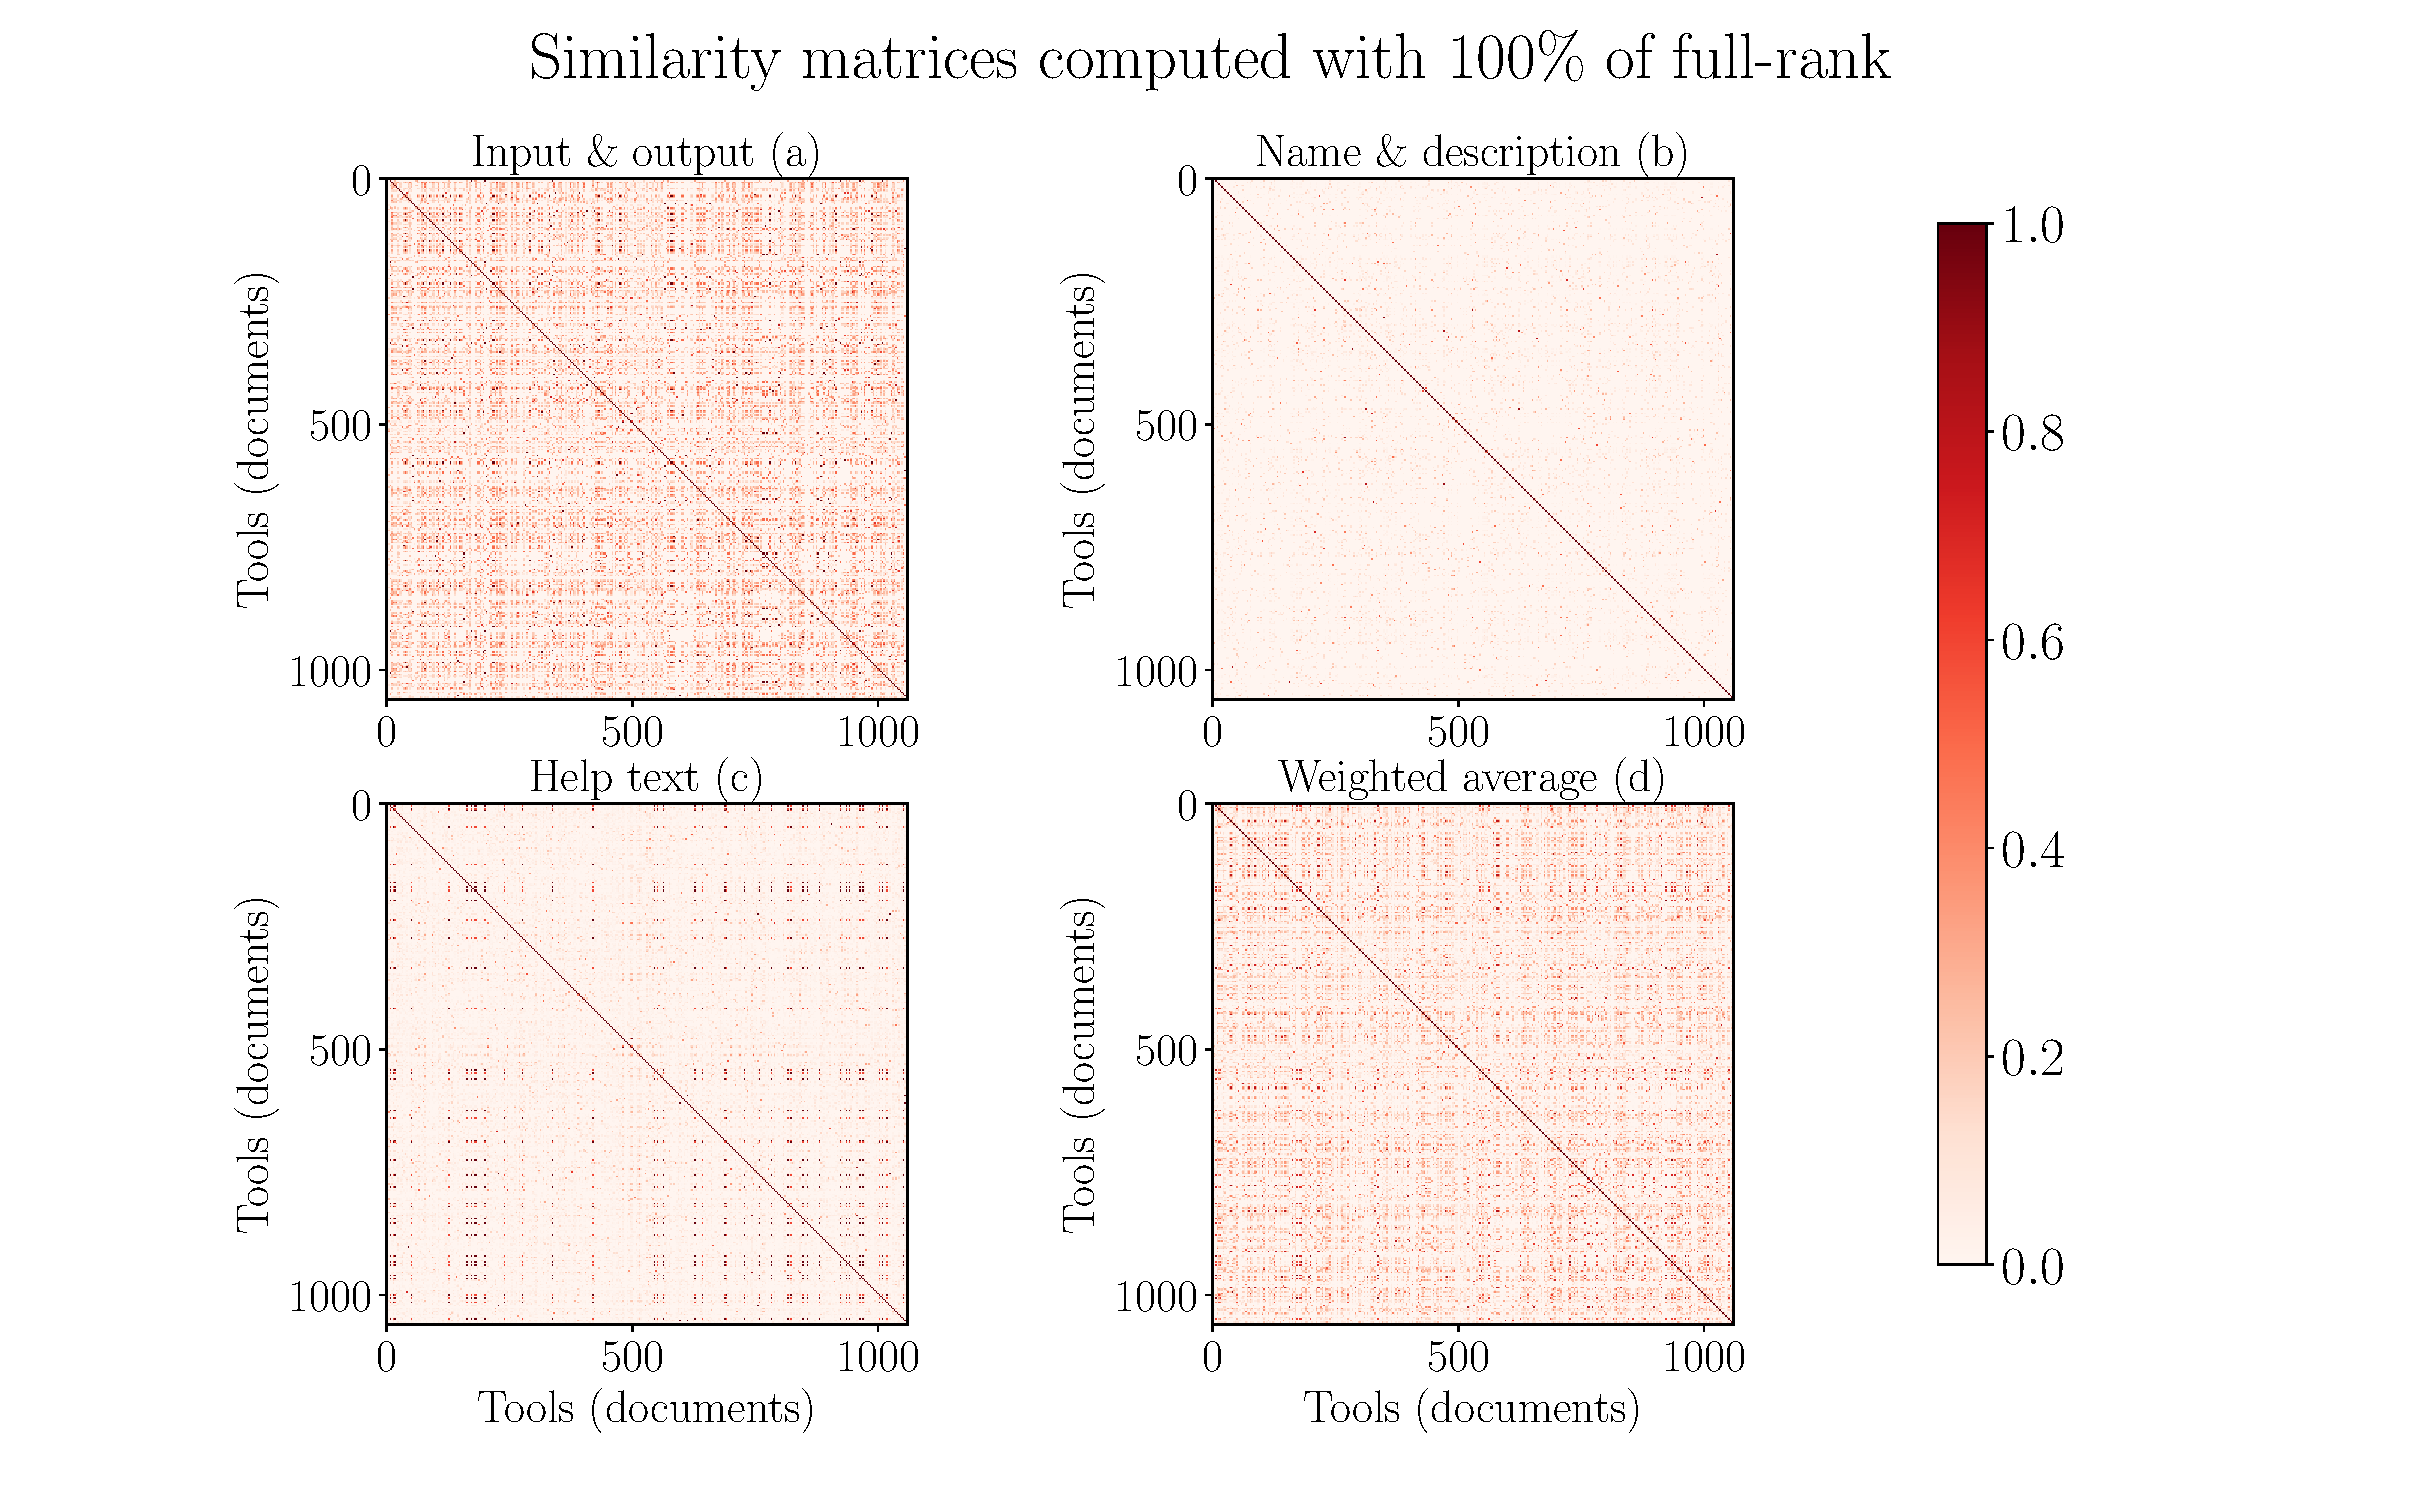
\includegraphics[scale=0.4]{figures/Similarity_matrices_100.pdf}}
    \caption[Similarity matrices computed using full-rank document-tokens matrices]{\textbf{Similarity matrices computed using full-rank documents-tokens matrices}: The heatmap shows documents-documents (tools-tools) correlation matrices for input and output file types (a), name and description (b) and help text (c) attributes. Subplot (d) shows a documents-documents (tools-tools) similarity (correlation) matrix which is the weighted average of similarity matrices computed in (a), (b) and (c) and applying weights (figure 18) learned by the gradient descent optimizer with momentum and accelerated gradient (equation 27 and 28). The corresponding documents-tokens matrices contain their full-ranks.}
\end{centering}
\end{figure}

\begin{figure}[h]
\begin{centering}
    {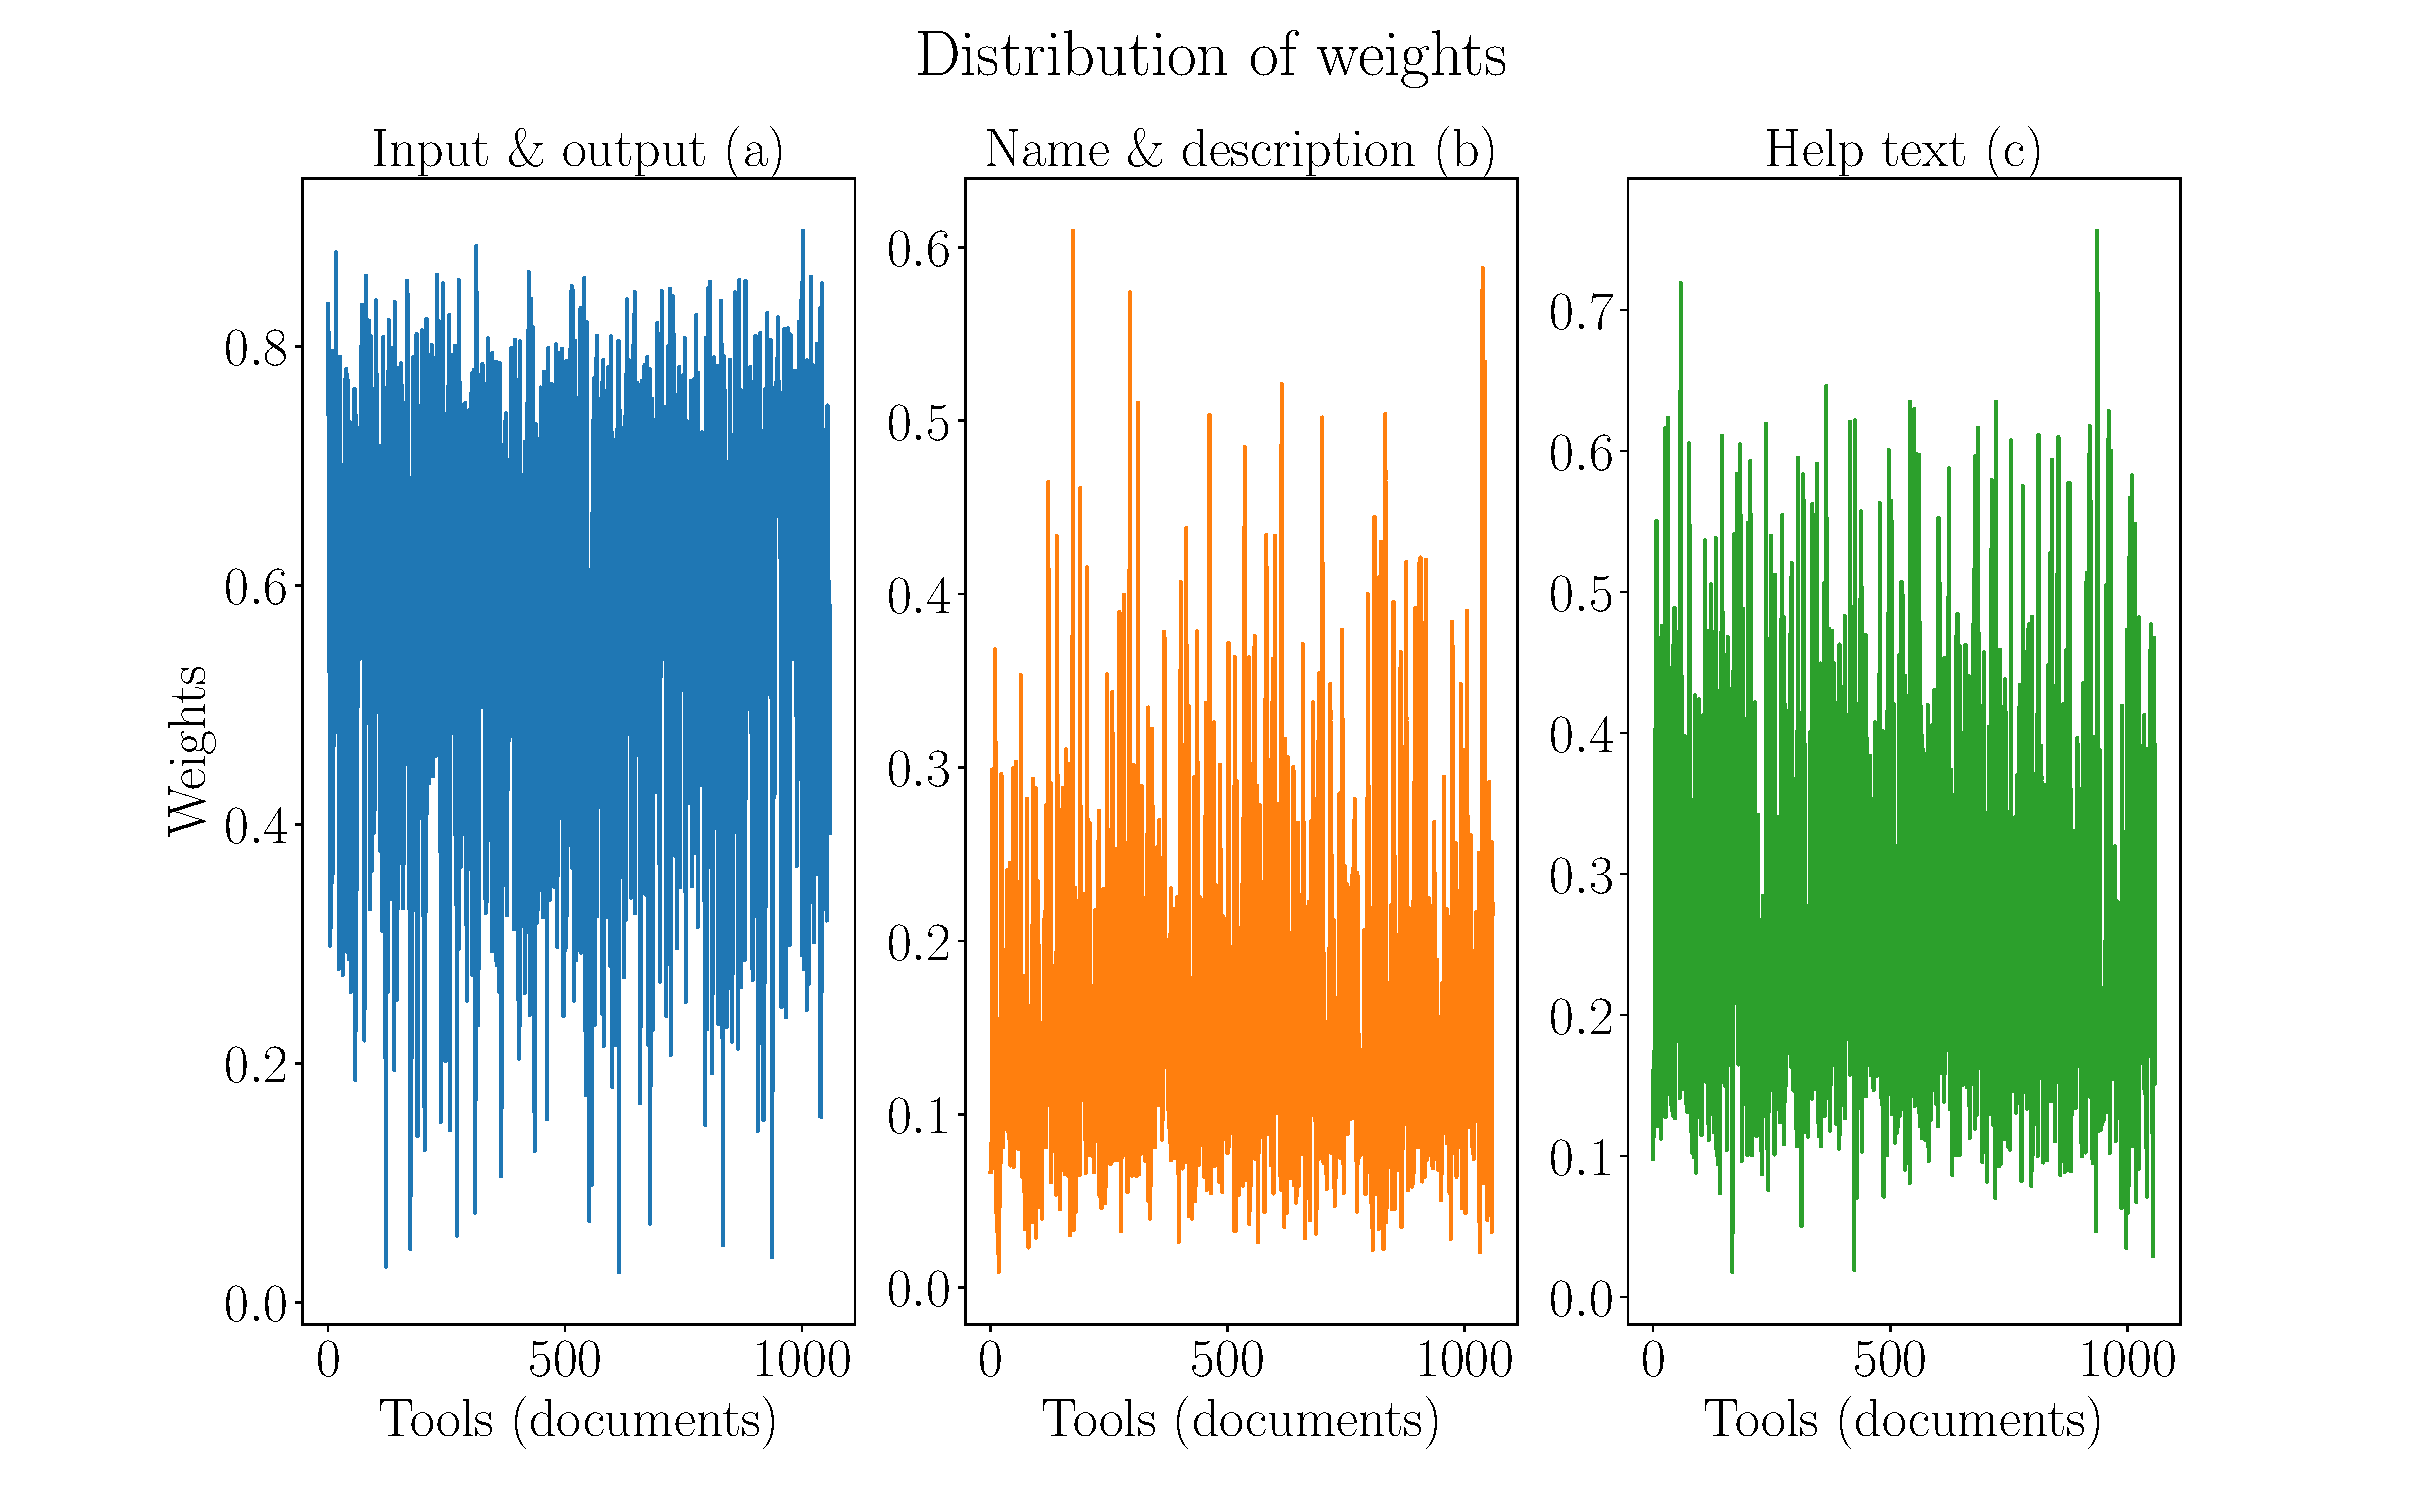
\includegraphics[scale=0.37]{figures/Weights_100.pdf}}
    \caption[Distribution of weights learned for similarity matrices computed using full-rank documents-tokens matrices]{\textbf{Distribution of weights learned for similarity matrices computed using full-rank documents-tokens matrices}: The plot shows the distribution of weights learned on the similarity matrices (17a, 17b and 17c) by the gradient descent optimizer for the input and output file types (a), name and description (b) and help text (c) attributes. The corresponding documents-tokens matrices contain their full-ranks.}
\end{centering}
\end{figure}

\subsection{70\% of full-rank}
In figure 17, we can see that the similarity matrices for name and description and help text are sparse. To reduce the sparsity,  we attempted to reduce the ranks of the respective documents-tokens matrices of these two attributes to 70\% of full-rank. For example, if the rank of a matrix is 100, we reduce the rank to 70 using singular value decomposition (equation 8). Along with reducing the ranks, we consequently reduced the singular values of these matrices as well (figure 11). Comparing figures 17 and 19, we see that the name and description and help text similarity matrices start becoming denser. The distribution of the weights also changes (figures 18 and 20). At this stage, it is hard to see the effect of rank reduction. Further, we reduced the ranks drastically to see the effect.

\begin{figure}[h]
\begin{centering}
    {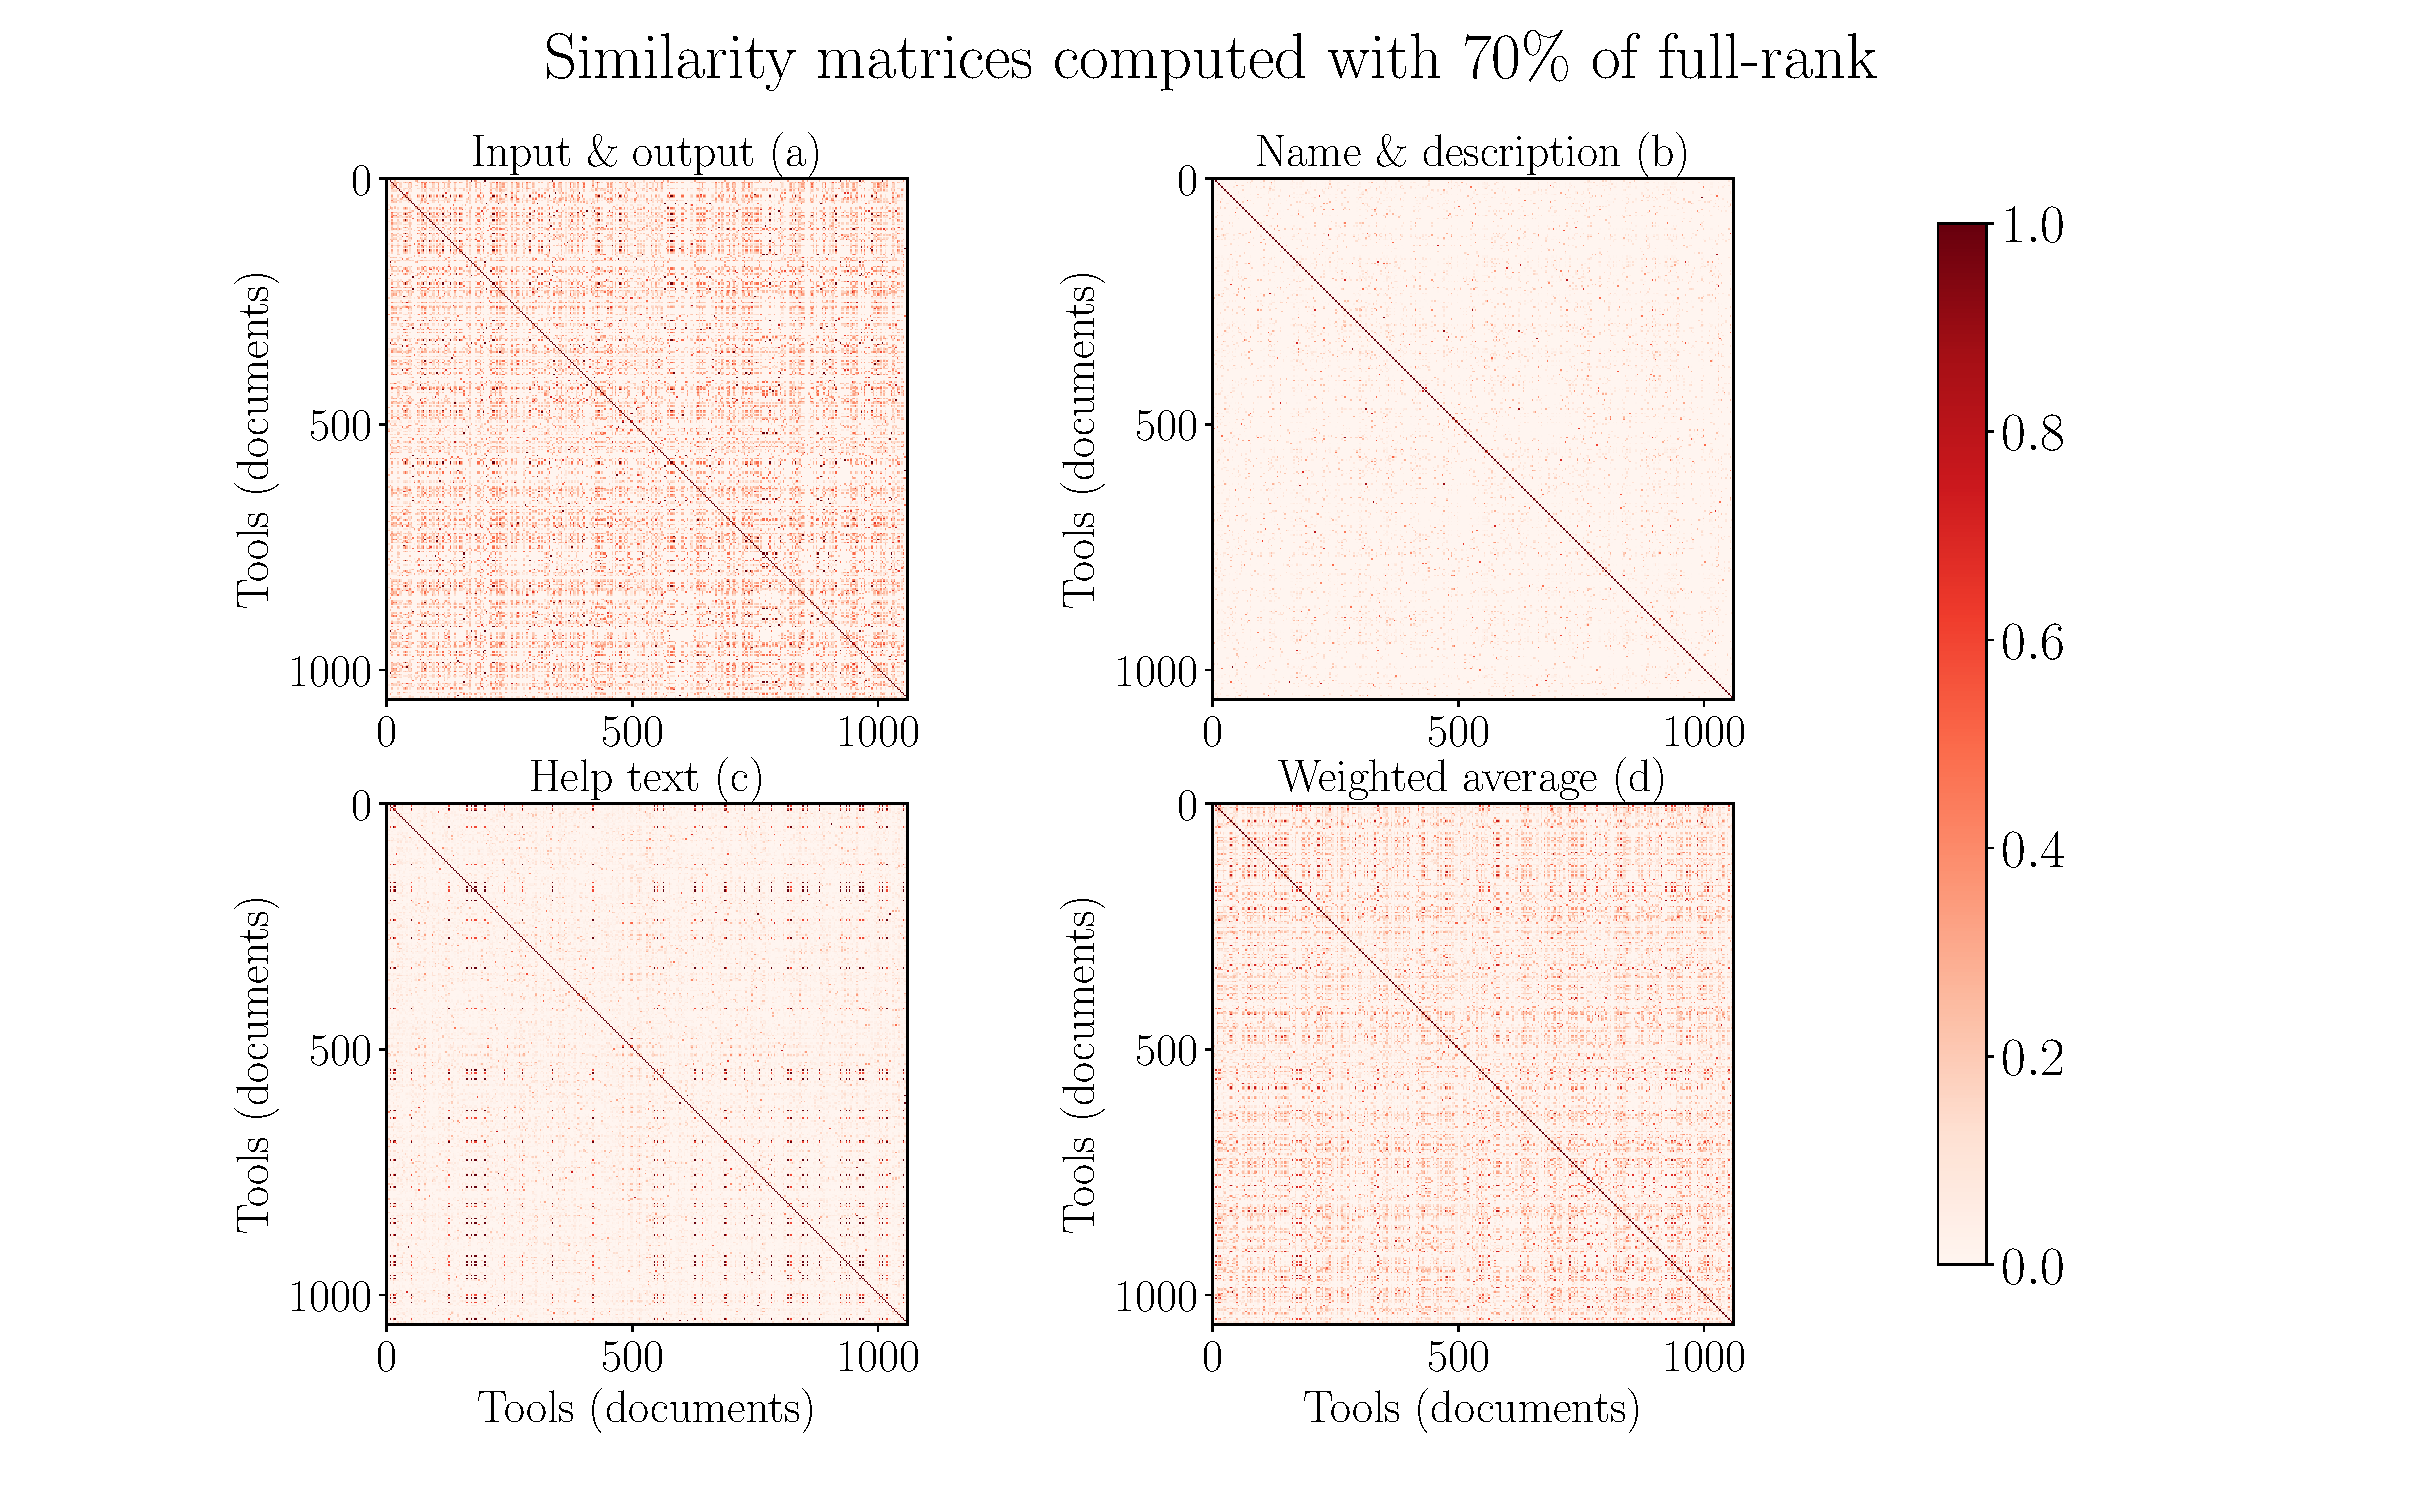
\includegraphics[scale=0.4]{figures/Similarity_matrices_070.pdf}}
    \caption[Similarity matrices computed using document-tokens matrices reduced to 70\% of their full-rank]{\textbf{Similarity matrices using 70\% of full-rank}: The heatmap shows documents-documents (tools-tools) correlation matrices for input and output (a), name and description (b) and help text (c) attributes. The (d) shows a documents-documents (tools-tools) correlation matrix which is the weighted average computed using (a), (b) and (c) and weights (figure 20) given by the gradient descent optimizer (equation 27). The corresponding documents-tokens matrices are reduced to 70\% of their respective full-ranks.}
\end{centering}
\end{figure}

\begin{figure}[h]
\begin{centering}
    {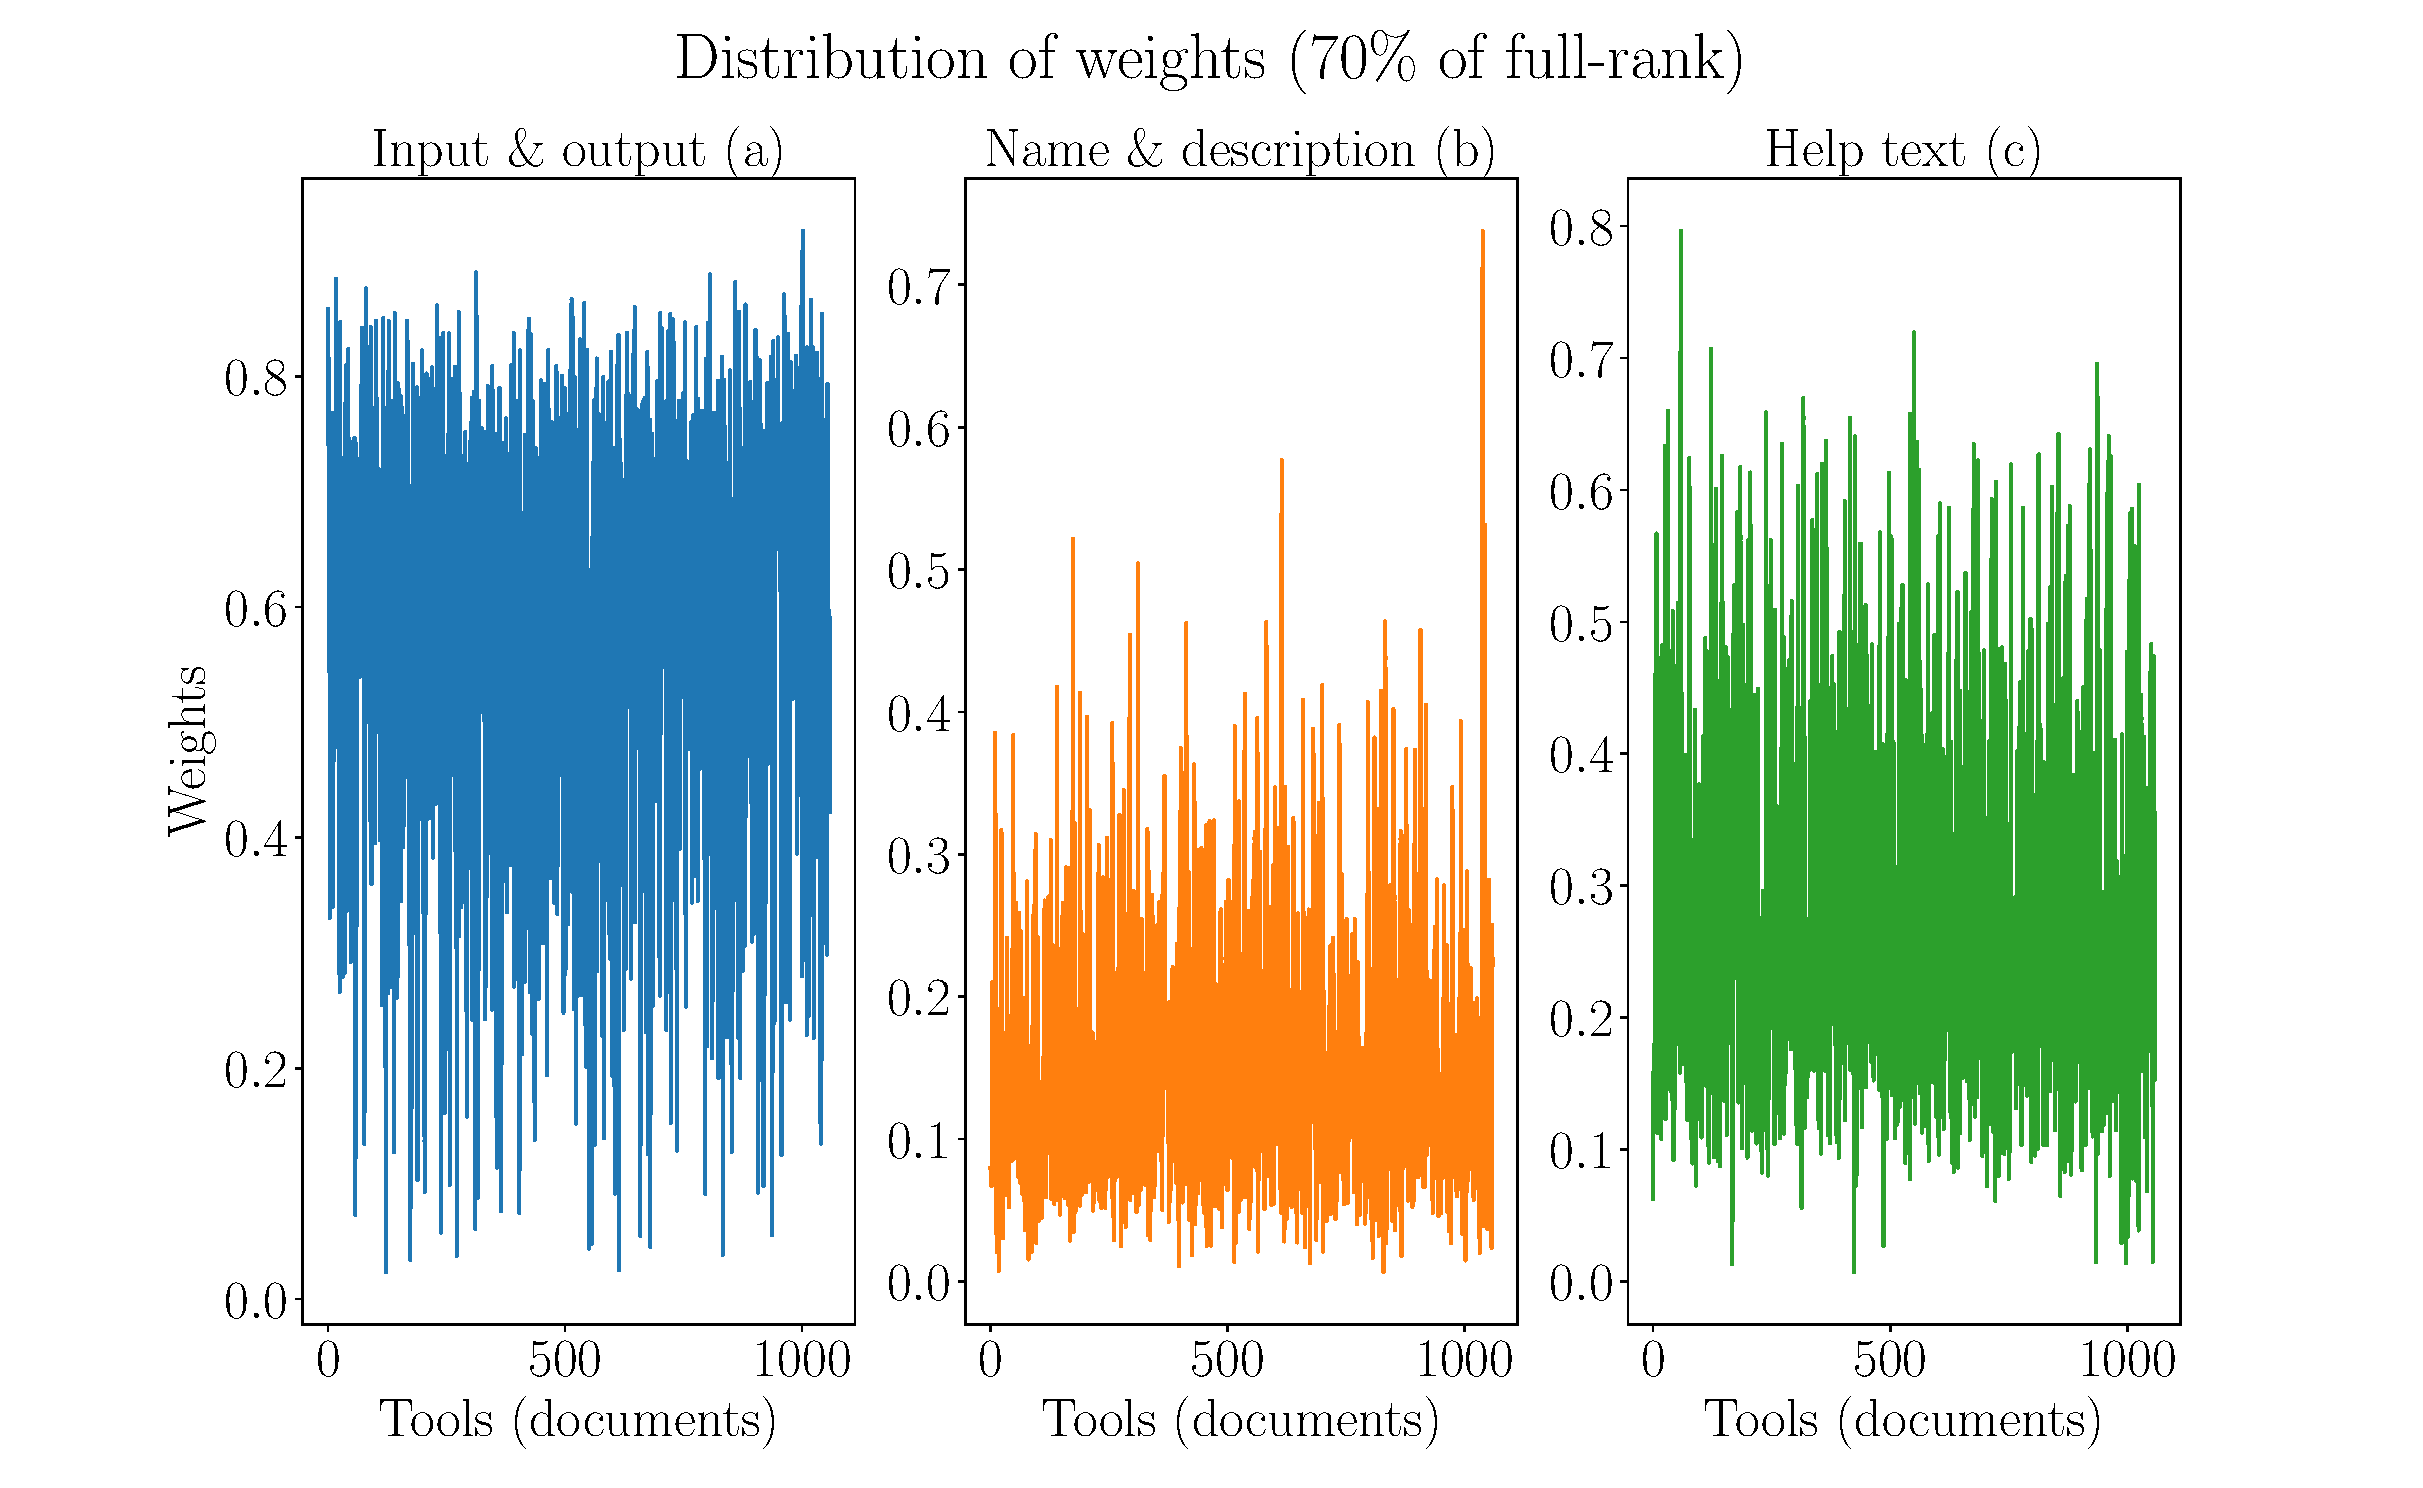
\includegraphics[scale=0.37]{figures/Weights_070.pdf}}
    \caption[Distribution of weights learned for similarity matrices computed using documents-tokens matrices reduced to $70\%$ of their full-rank]{\textbf{Distribution of weights learned for similarity matrices computed using documents-tokens matrices reduced to $70\%$ of their full-rank}: The plot shows the distribution of weights learned on the similarity matrices (19a, 19b and 19c) by the gradient descent optimizer for the input and output file types (a), name and description (b) and help text (c) attributes. The corresponding documents-tokens matrices contain $70\%$ of their full-ranks.}
\end{centering}
\end{figure}

\subsection{30\% of full-rank}
To see the effect of rank reduction, we reduced the ranks of two documents-tokens matrices further to $30\%$ of full-rank. This is a large reduction and would amount to keeping $\approx 60\%$ (removing $\approx 40\%$) (figure 11) of the sum of singular values for all the documents-tokens matrices. In figures 21 and 22, the effect of rank reduction is more visible compared to $70\%$ (figures 19 and 20). We see that the magnitude of weights learned for input and output files starts to decrease and the magnitude of weights for name and description and help text start to increase (figure 22) because the corresponding similarity matrices score become denser (figure 21).

\begin{figure}[h]
\begin{centering}
    {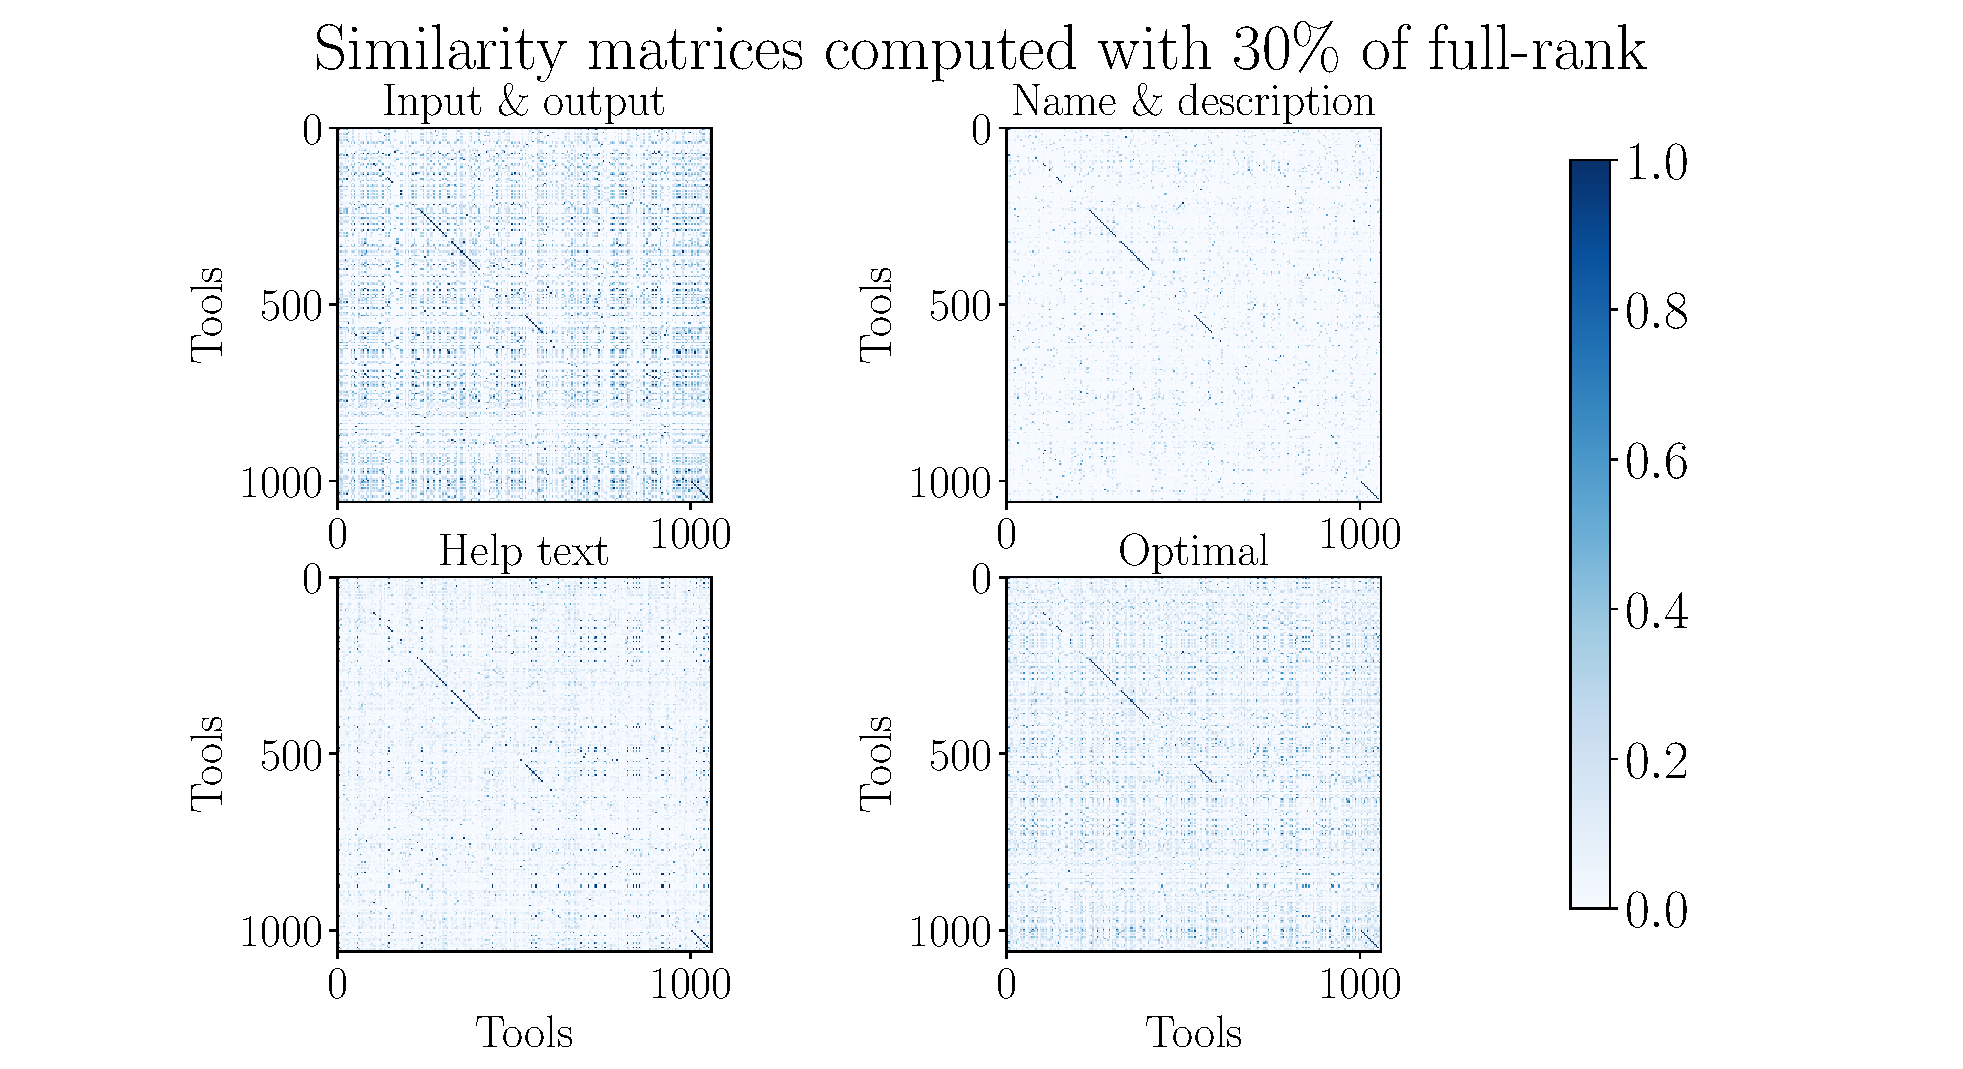
\includegraphics[scale=0.4]{figures/Similarity_matrices_030.pdf}}
    \caption[Similarity matrices computed using document-tokens matrices reduced to $30\%$ of their full-rank]{\textbf{Similarity matrices computed using document-tokens matrices reduced to $30\%$ of their full-rank}: The heatmap shows documents-documents (tools-tools) correlation matrices for input and output (a), name and description (b) and help text (c) attributes. The (d) shows a documents-documents (tools-tools) correlation matrix which is the weighted average computed using (a), (b) and (c) and weights (figure 22) given by the gradient descent optimizer (equation 15). The corresponding documents-tokens matrices are reduced to $30\%$ of their respective full-ranks.}
\end{centering}
\end{figure}

\begin{figure}[h]
\begin{centering}
    {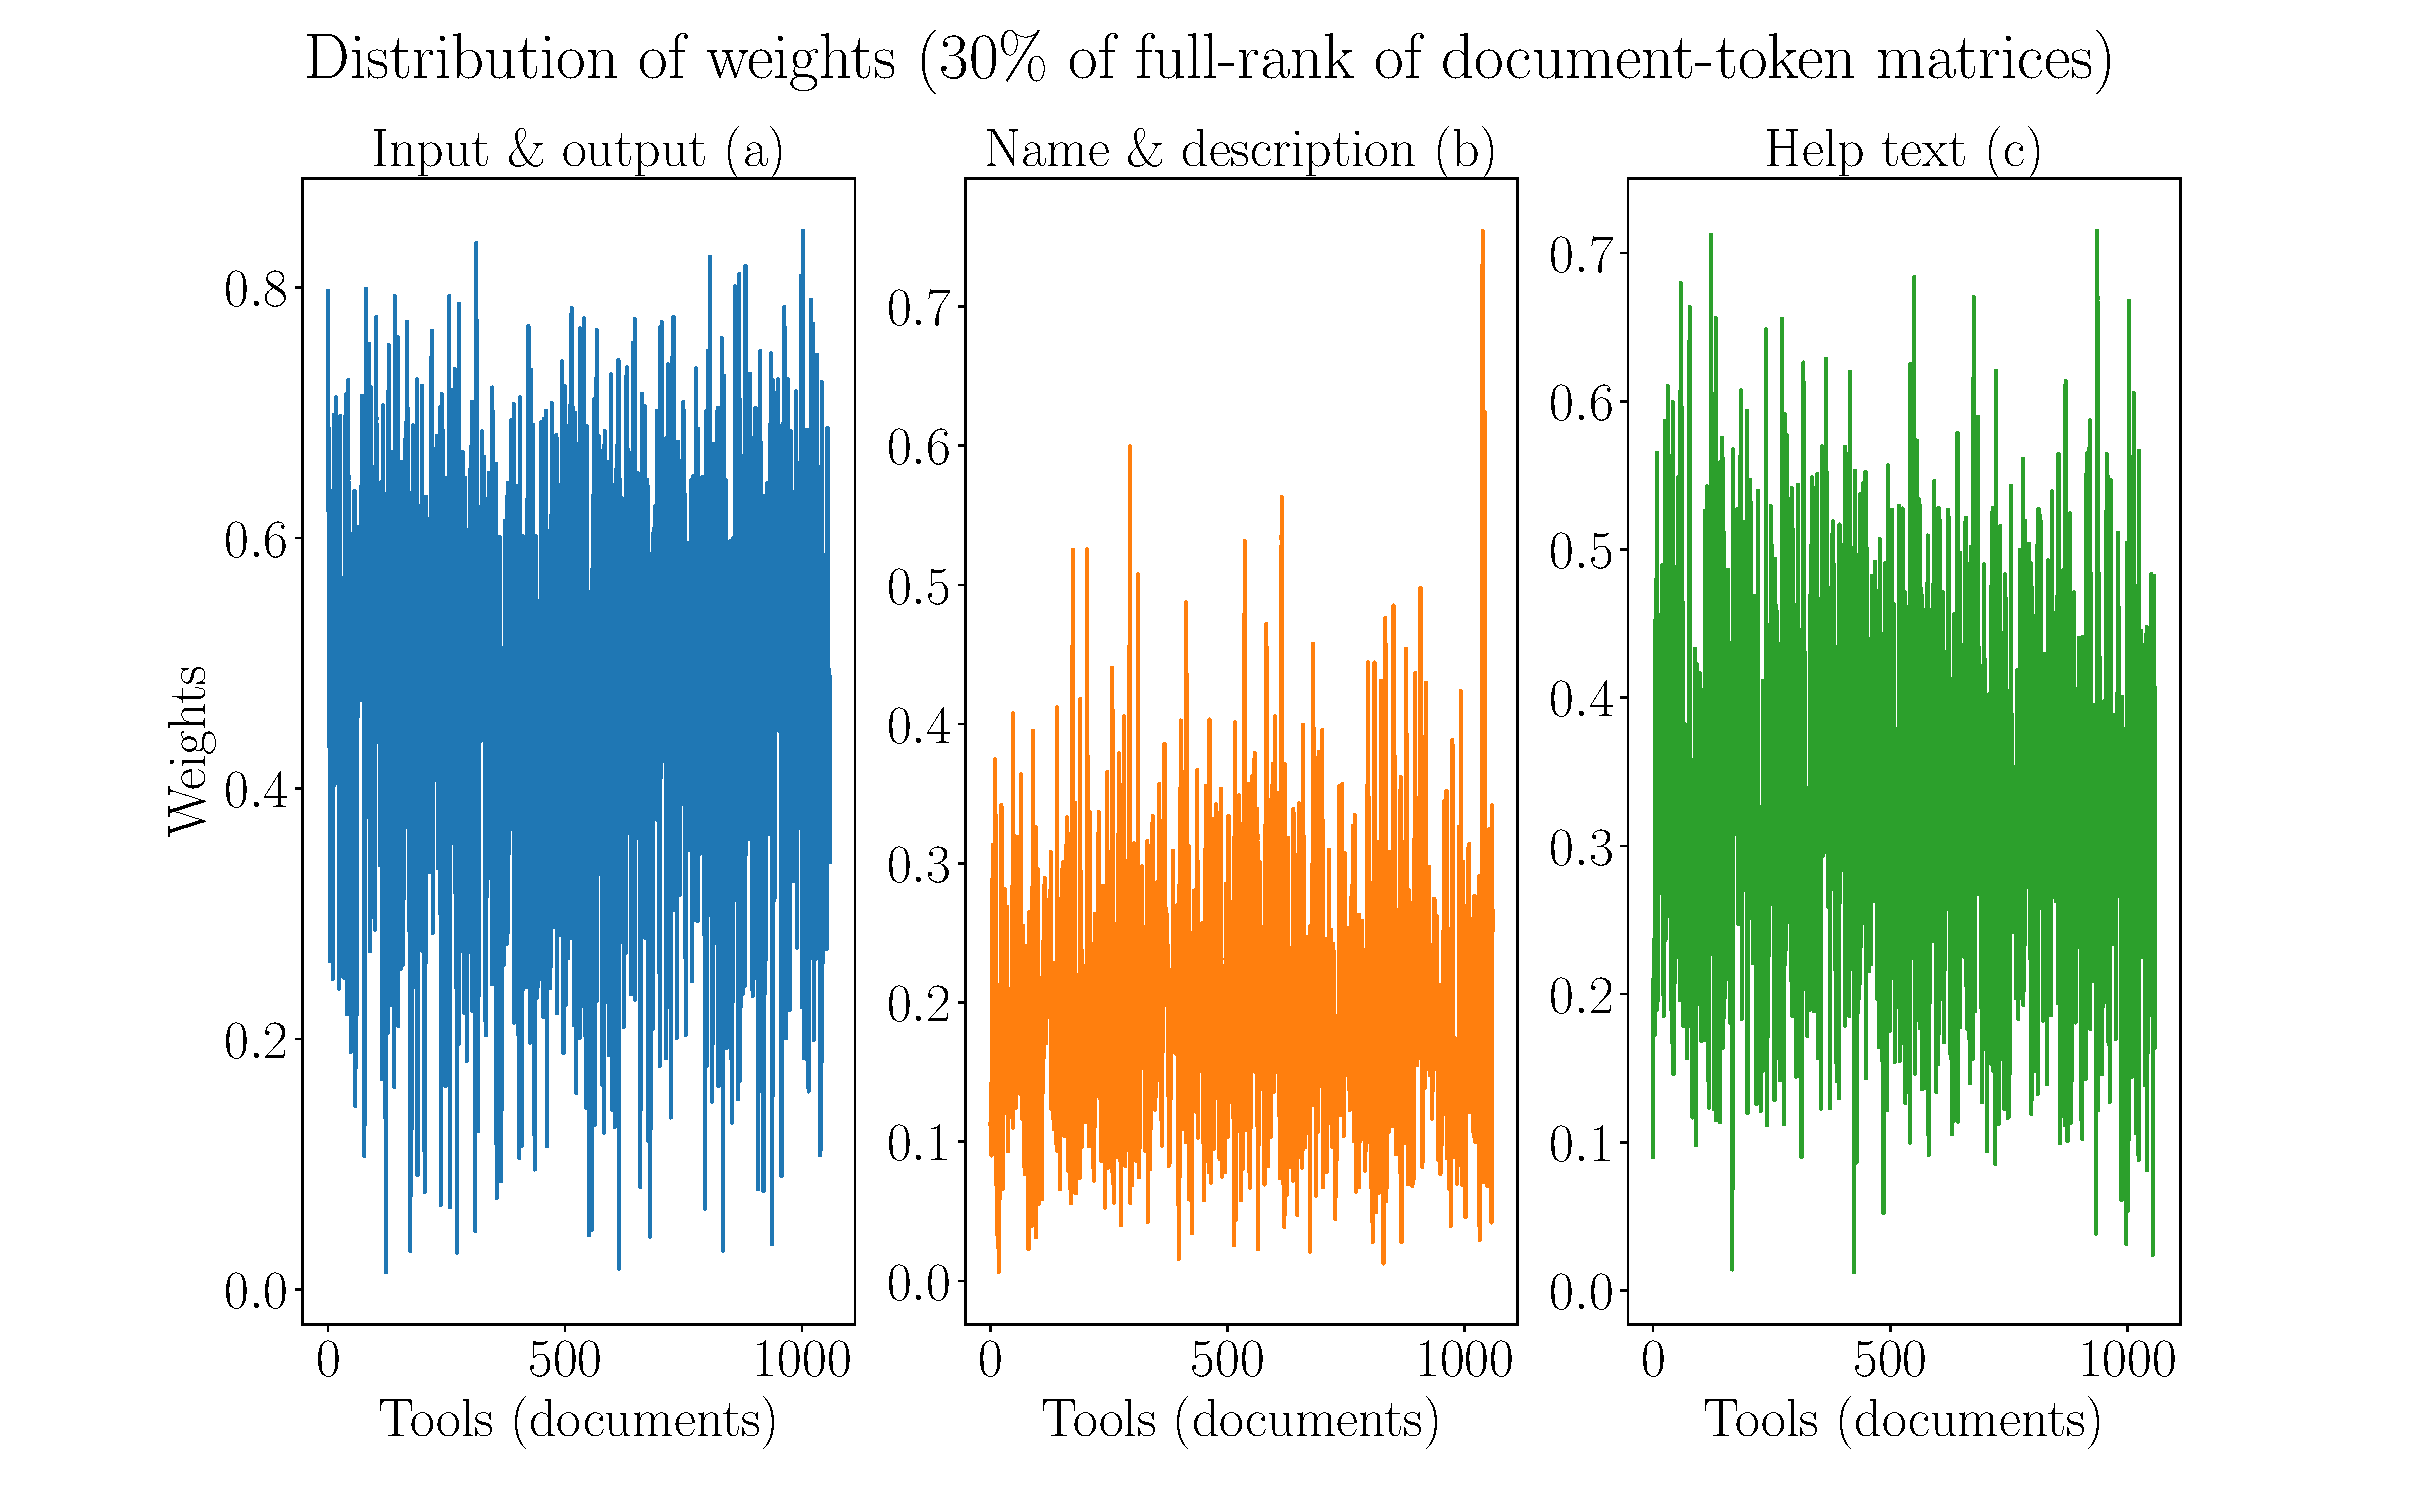
\includegraphics[scale=0.37]{figures/Weights_030.pdf}}
    \caption[Distribution of weights learned for similarity matrices computed using documents-tokens matrices reduced to $30\%$ of their full-rank]{\textbf{Distribution of weights learned for similarity matrices computed using documents-tokens matrices reduced to $30\%$ of their full-rank}: The plot shows the distribution of weights learned on the similarity matrices (21a, 21b and 21c) by the gradient descent optimizer for the input and output file types (a), name and description (b) and help text (c) attributes. The corresponding documents-tokens matrices contain $30\%$ of their full-ranks.}
\end{centering}
\end{figure}

\subsection{5\% of full-rank}
Further, we reduced the ranks of two documents-tokens matrices to $5\%$ of their full-ranks. By choosing this low value, we considered only top $\approx 20\%$ of the sum of singular values (figure 11). From figure 23, we can see that all the similarity matrices corresponding to the attributes are denser compared to figures 17, 91 and 21. Due to this, the weights distribution also changes (figure 24). We learn higher weights for name and description (24b) and help text (24c) compared to the weights for input and output file types (24a).

\begin{figure}[h]
\begin{centering}
    {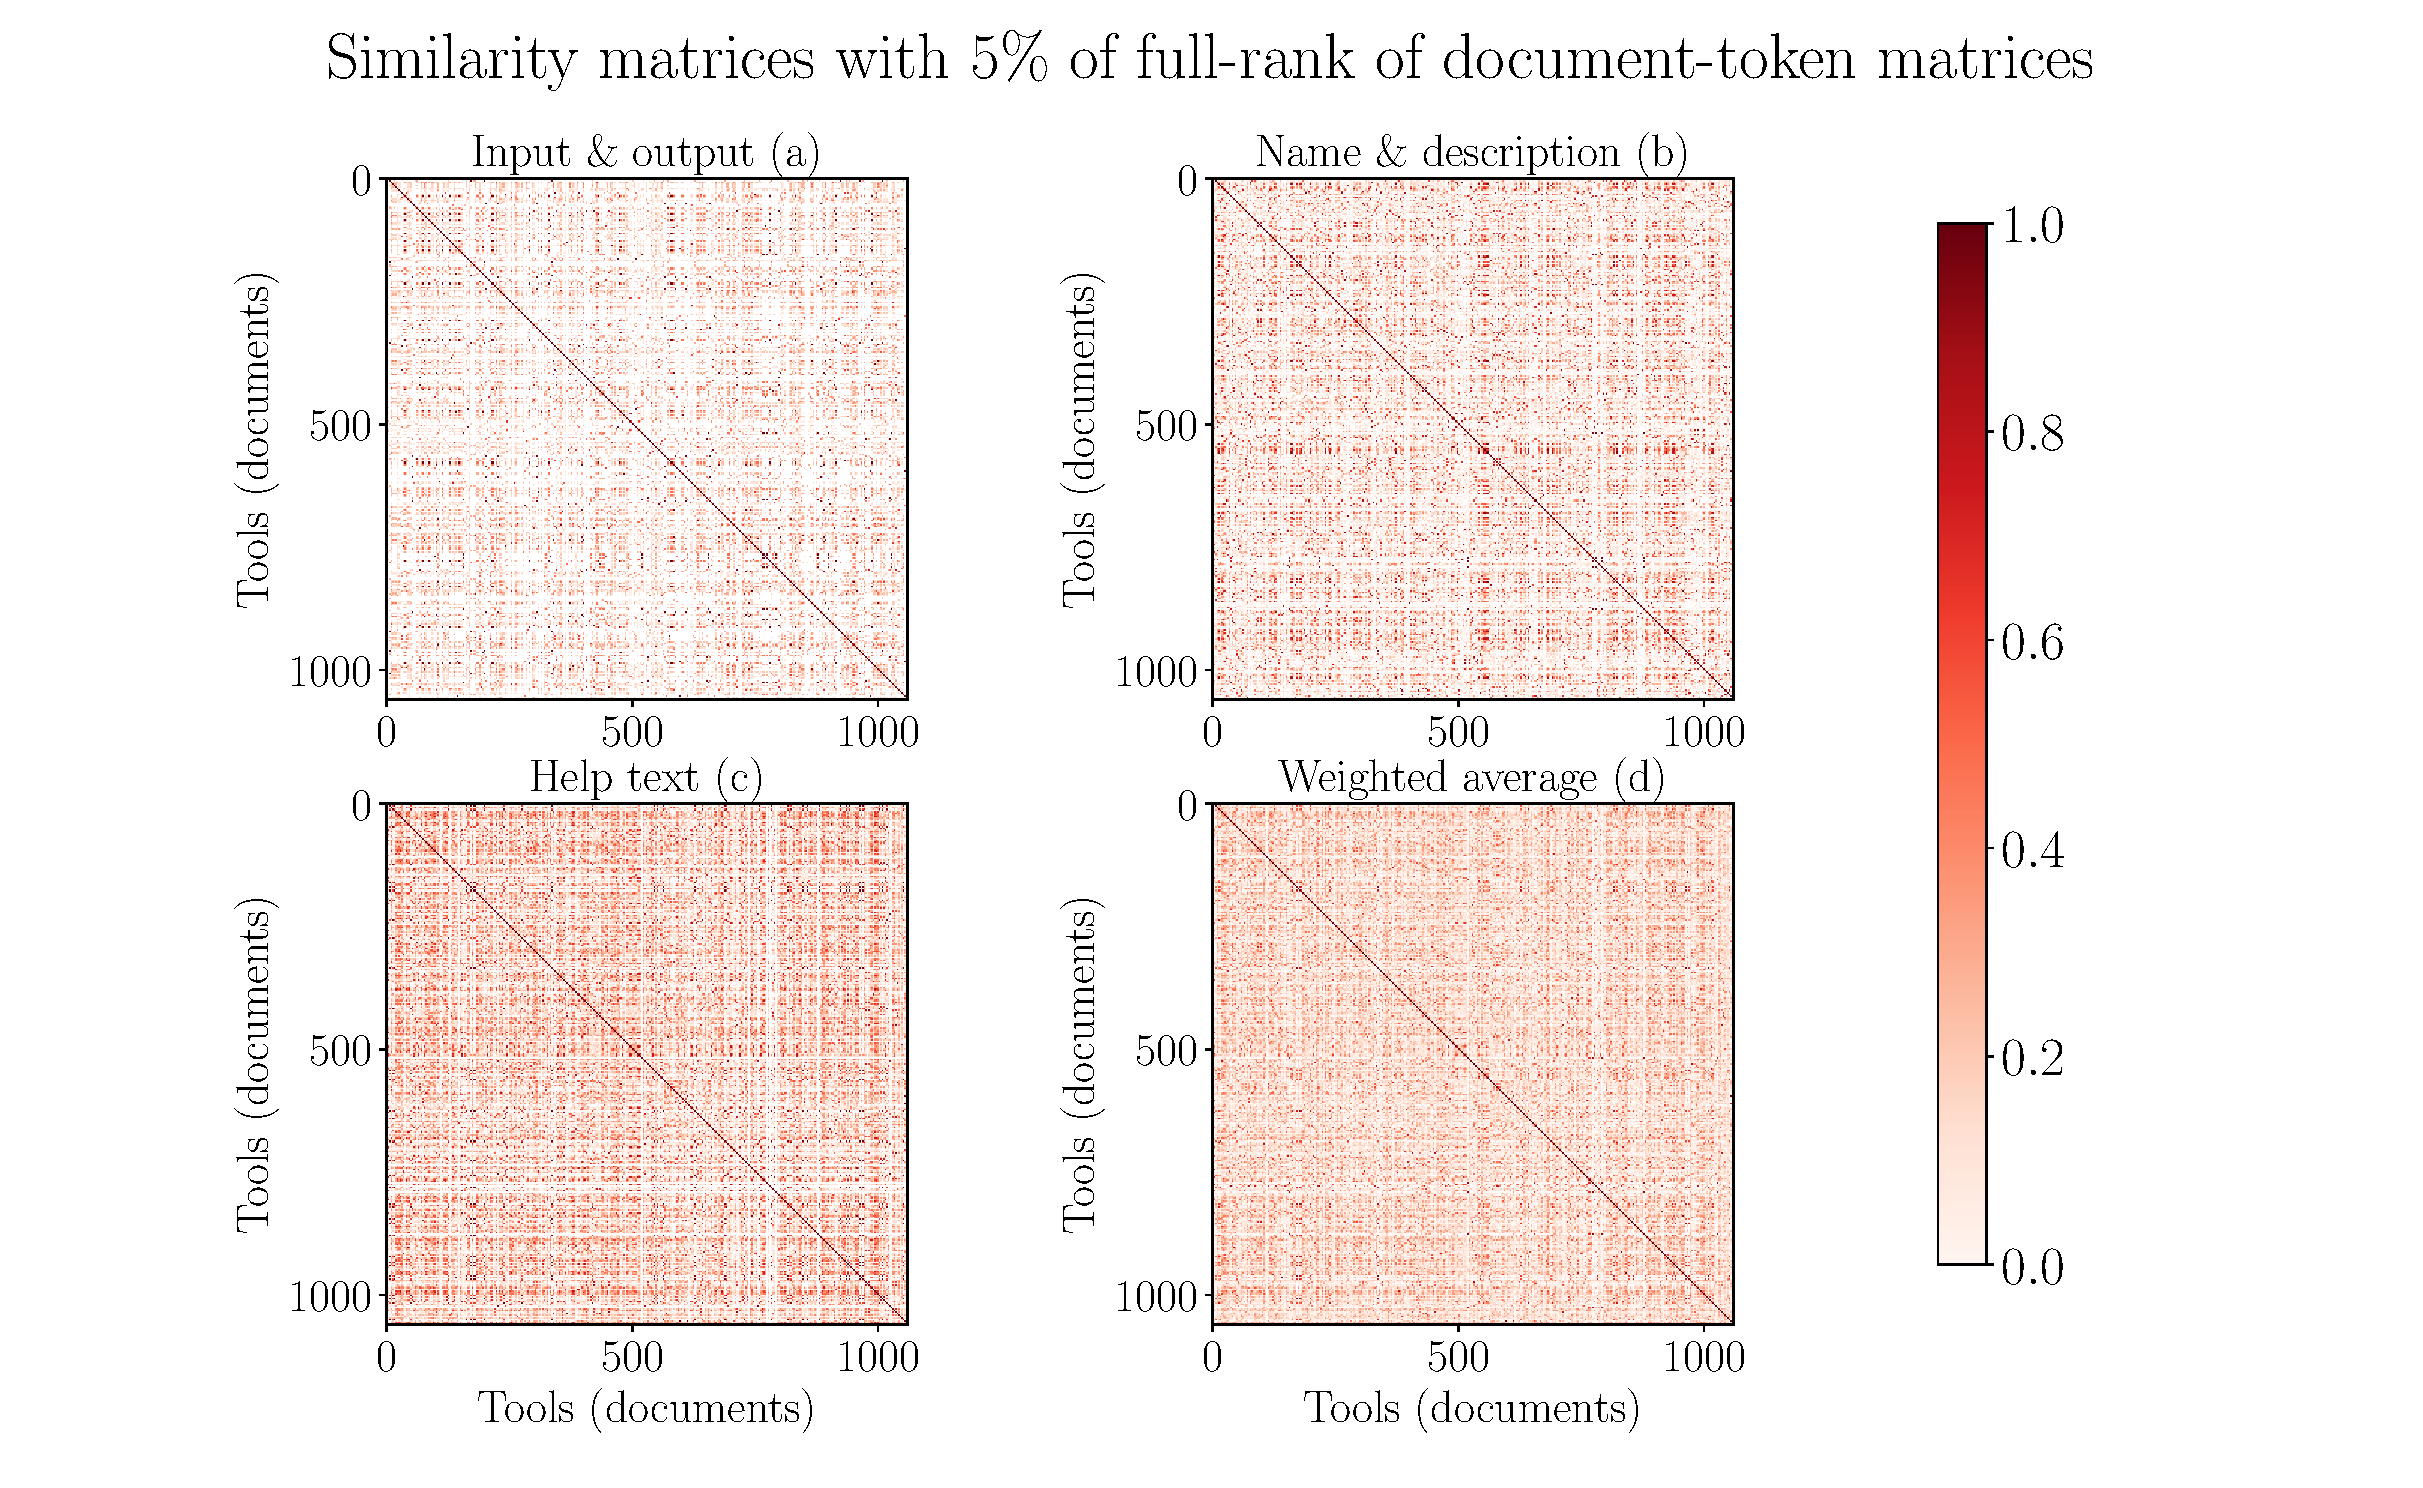
\includegraphics[scale=0.4]{figures/Similarity_matrices_005.pdf}}
    \caption[Similarity matrices computed using document-tokens matrices reduced to $5\%$ of their full-rank]{\textbf{Similarity matrices computed using document-tokens matrices reduced to $5\%$ of their full-rank}: The heatmap shows documents-documents (tools-tools) correlation matrices for input and output (a), name and description (b) and help text (c) attributes. The (d) shows a documents-documents (tools-tools) correlation matrix which is the weighted average computed using (a), (b) and (c) and weights (figure 24) given by the gradient descent optimizer (equation 15). The corresponding documents-tokens matrices are reduced to $5\%$ of their respective full-ranks.}
\end{centering}
\end{figure}

\begin{figure}[h]
\begin{centering}
    {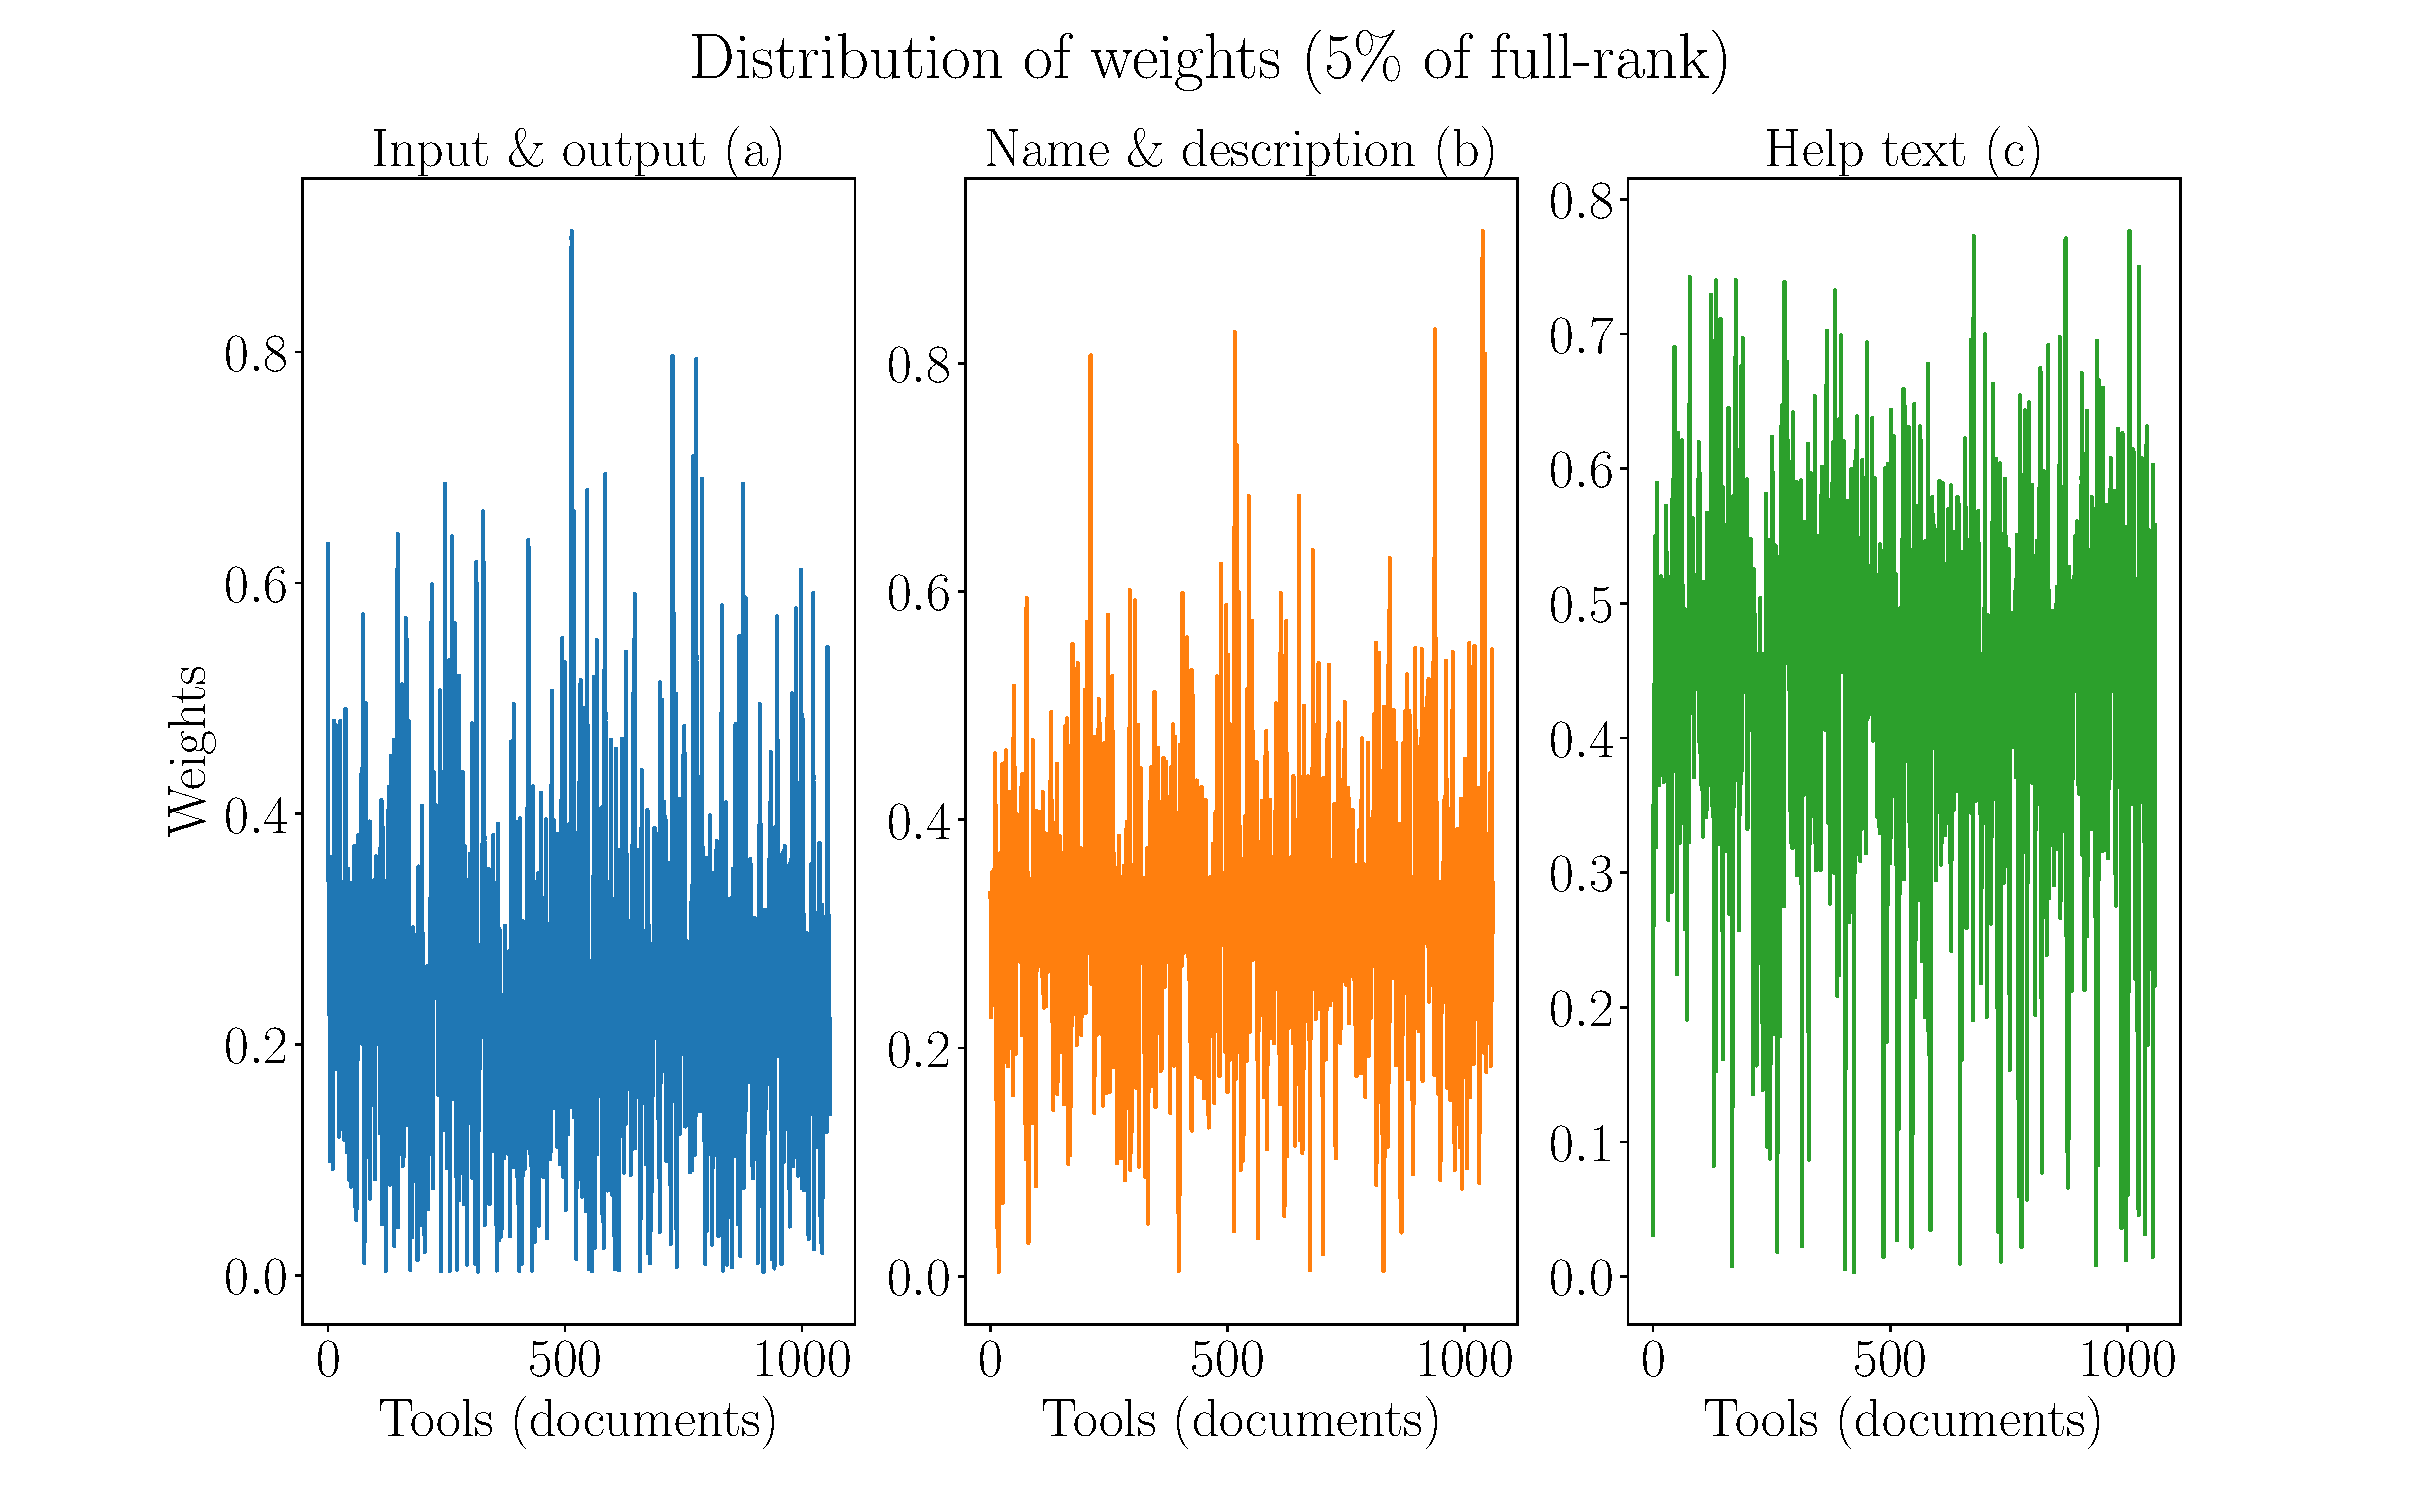
\includegraphics[scale=0.37]{figures/Weights_005.pdf}}
    \caption[Distribution of weights learned for similarity matrices computed using documents-tokens matrices reduced to $5\%$ of their full-rank]{\textbf{Distribution of weights learned for similarity matrices computed using documents-tokens matrices reduced to $5\%$ of their full-rank}: The plot shows the distribution of weights learned on the similarity matrices (23a, 23b and 23c) by the gradient descent optimizer for the input and output file types (a), name and description (b) and help text (c) attributes. The corresponding documents-tokens matrices contain $5\%$ of their full-ranks.}
\end{centering}
\end{figure}

\subsection{Improvement verification}
To verify that the matrix rank reduction actually works and learns better similarity scores for tools (documents) which are similar in the actual case, we showcase two ways. One idea is to show quantitatively the reduction in mean squared error. Another is to verify the similar tools and the corresponding weights using a static visualizer.

\subsubsection{Reduction in error}
We observe a drop in mean squared error when we decrease the ranks of the matrices (figure 25). When we reduce the ranks, the similarity scores for the name and description and help text increase. This increase accounts for their larger weights learned by the optimizer. The weights on an average become more balanced and together with higher similarity scores account for the decrease in the mean squared error. With decreasing mean squared error, the average similarity scores across all the tools using uniform and optimal weights increased. From figures 26 and 27, we find that the average similarity scores using uniform weights get better (from $\approx0.05$ to $\approx0.12$, mean of the orange lines in figures 26 and 27). The blue lines which measure the average similarity computed using optimal weights also record higher similarity (from $\approx0.075$ to $\approx0.15$, blue lines in figures 26 and 27). In the absence of true similarity values, it is hard to establish that we actually improve the performance. To be more certain that we improve the ranking of similar tools, we created a visualizer using javascript and html to look through the similar tools and their respective scores and weights for all tools. The next section explains it.

\begin{figure}[h]
\begin{centering}
    {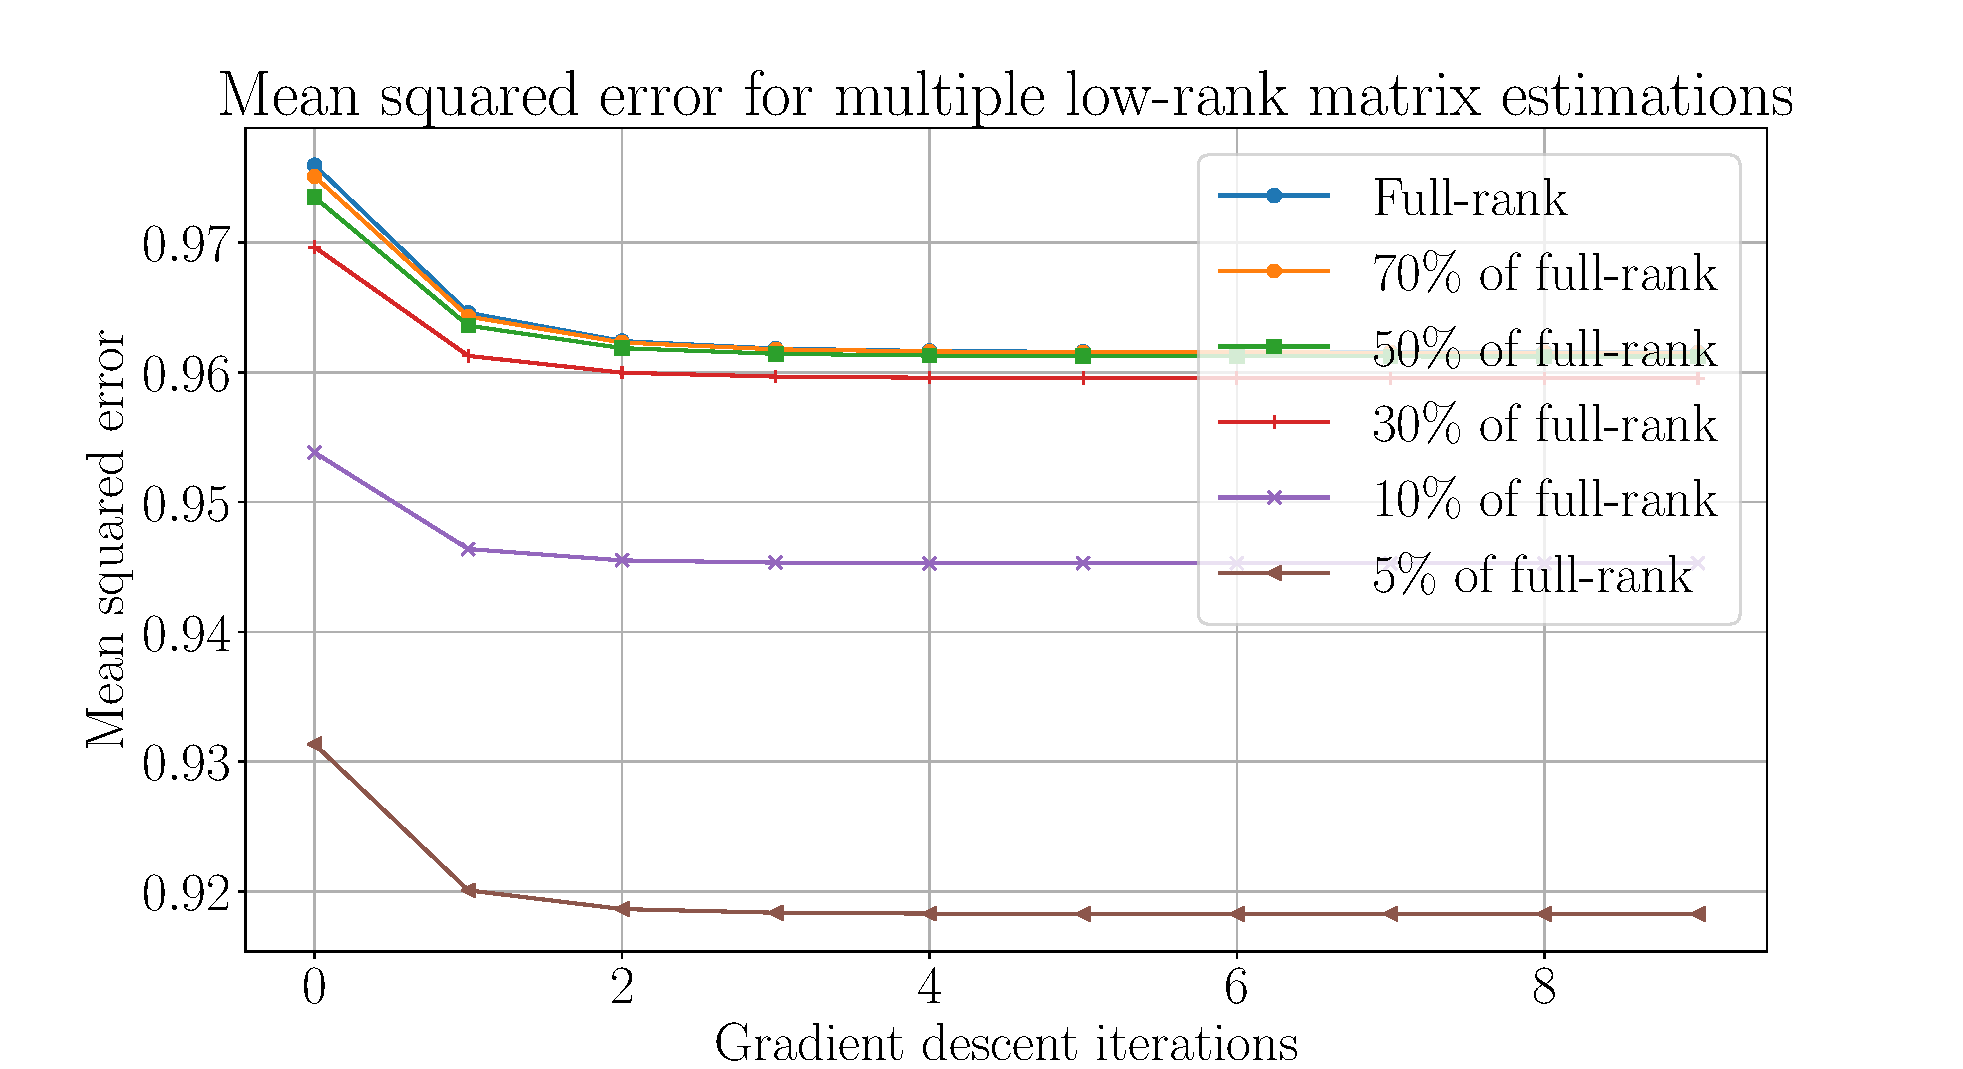
\includegraphics[scale=0.37]{figures/MSE_iterations_low_rank.pdf}}
    \caption[Mean squared error using full-rank and multiple estimations of low-rank (latent semantic analysis approach]{\textbf{Mean squared error using full-rank and multiple estimations of low-rank (latent semantic analysis approach) documents-tokens matrices}: The line plot shows a comparison of mean squared error computed separately using full-rank and multiple estimations of low-rank documents-tokens matrices. Each line shows an average error over all the tools and attributes which drops and becomes stable as we move along the iterations of gradient descent.}
\end{centering}
\end{figure}

\begin{figure}[h]
\begin{centering}
    {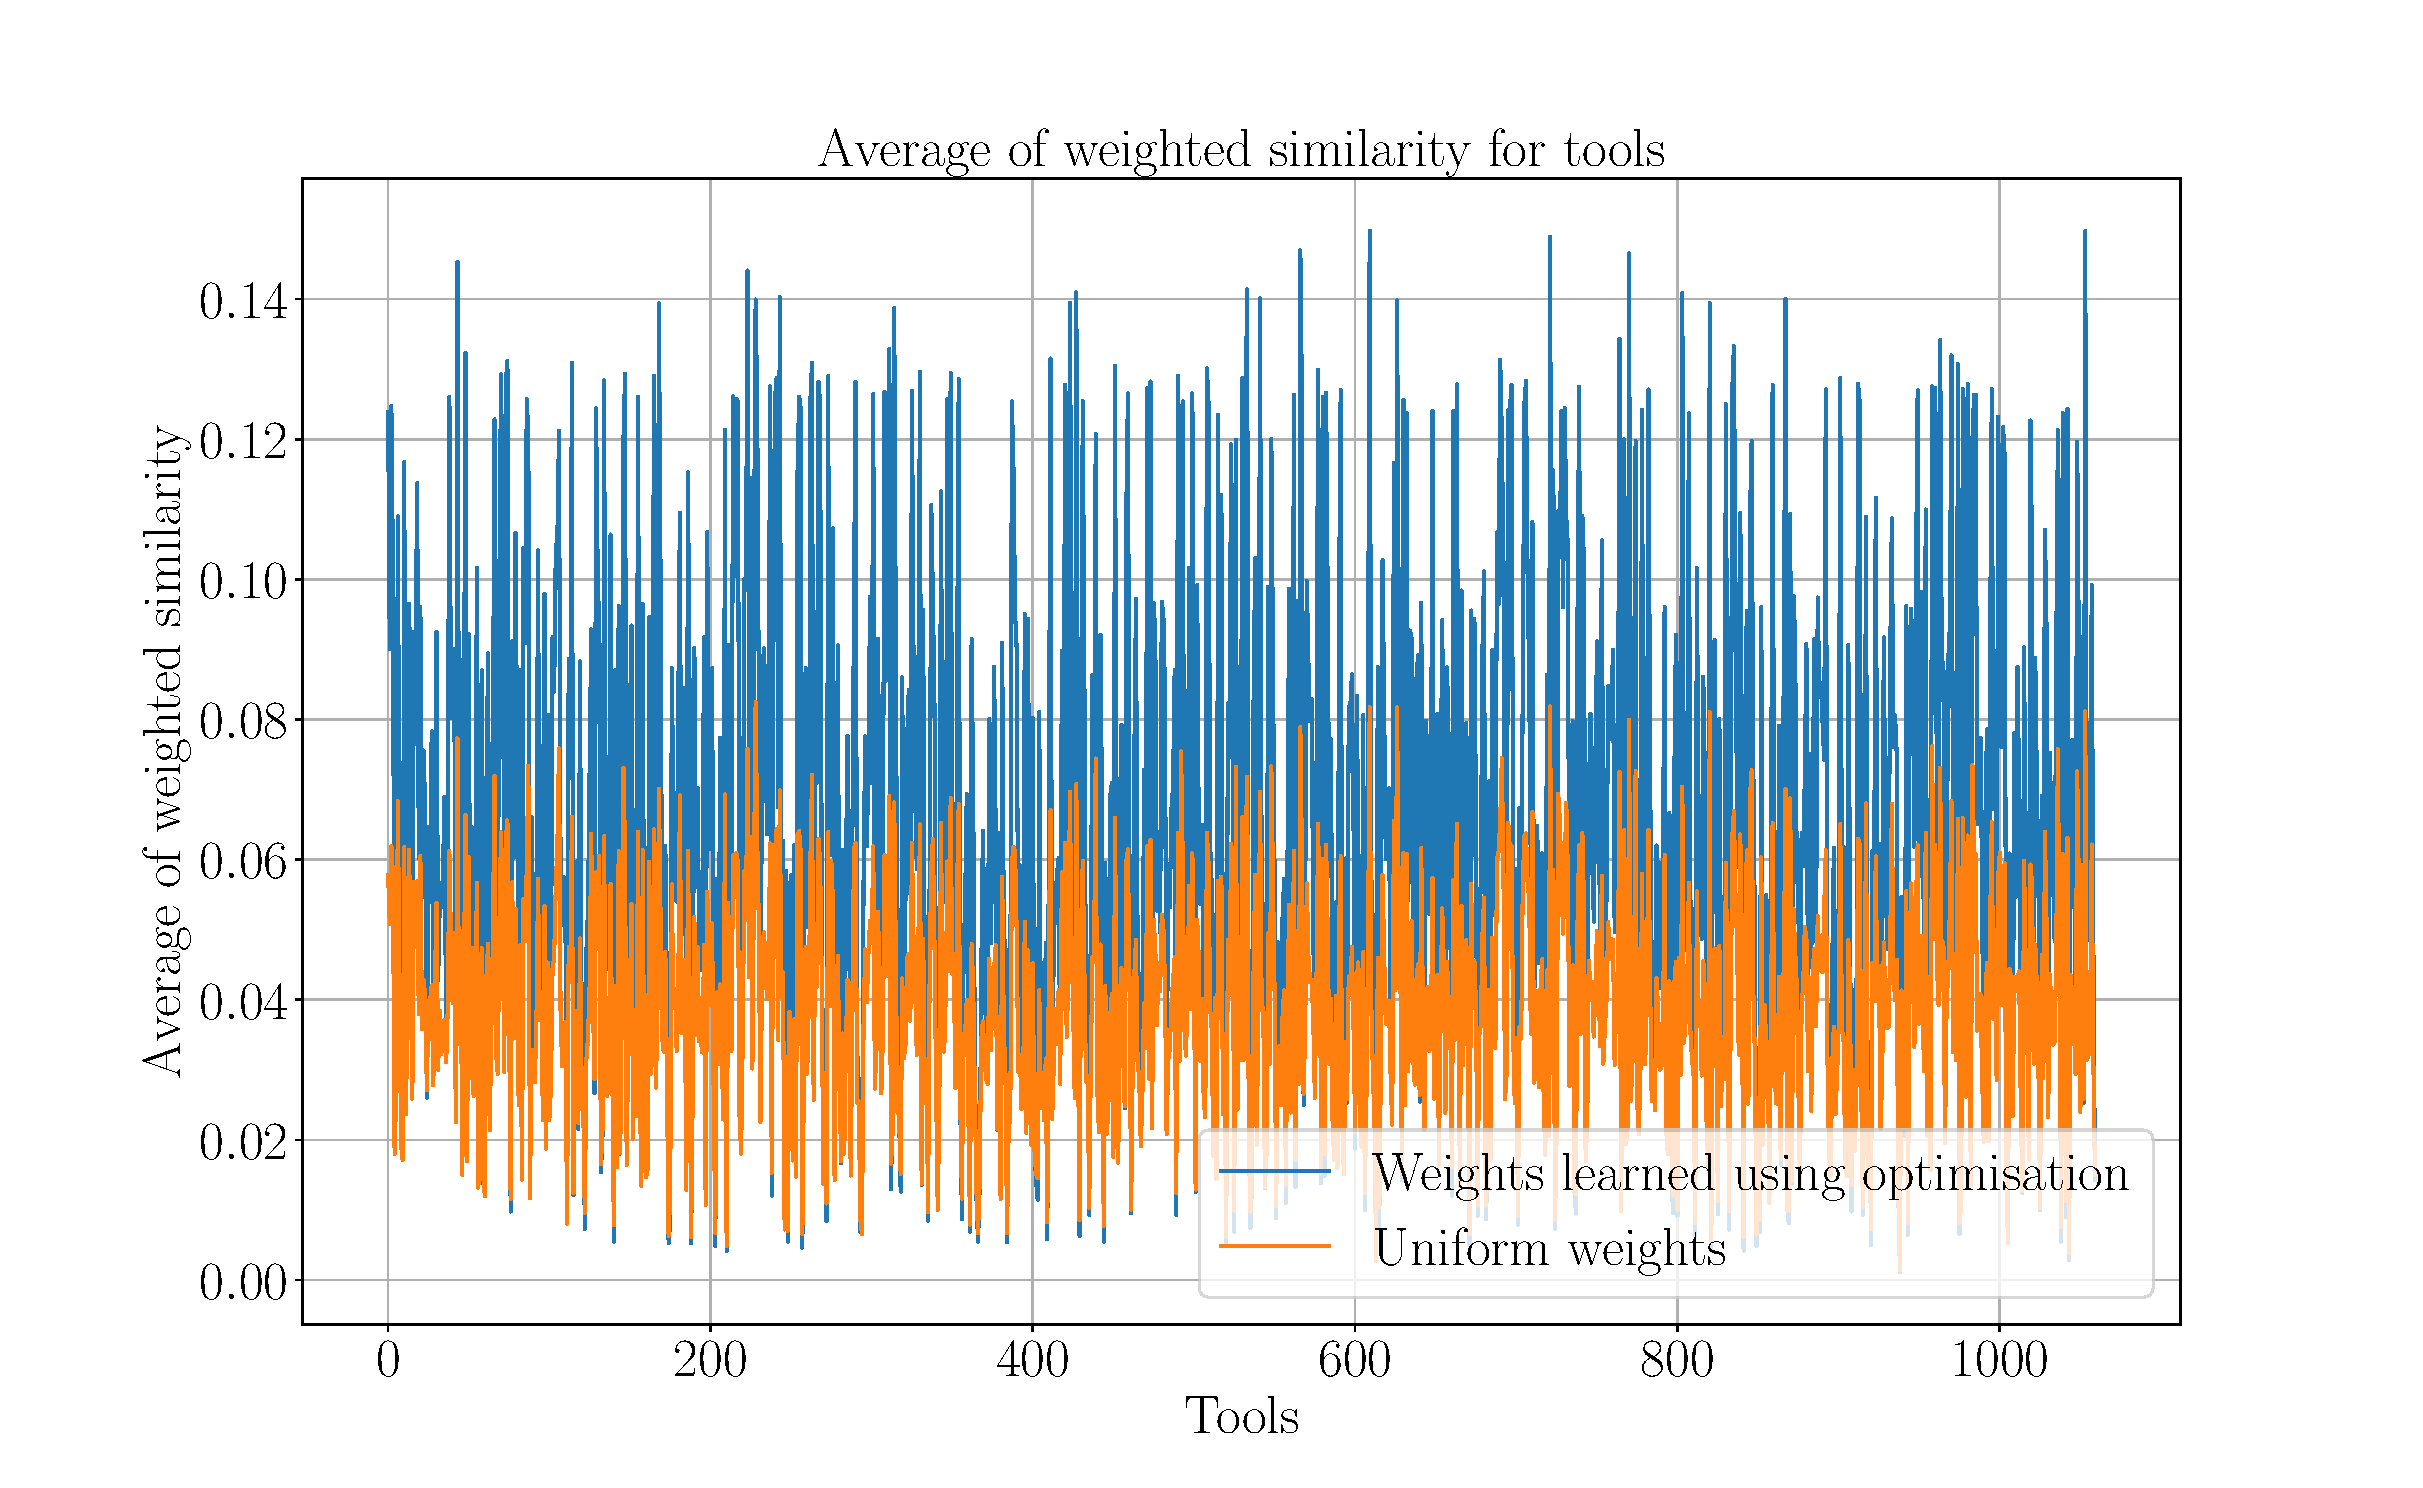
\includegraphics[scale=0.37]{figures/Optimization_100_lsi.pdf}}
    \caption[Average of uniformly and optimally weighted similarity scores computed using full-rank documents-tokens matrices across all tools]{\textbf{Average of uniformly and optimally weighted similarity scores computed using full-rank documents-tokens matrices across all tools}: The plot shows the average similarity scores where full-rank documents-tokens matrices are used to compute similarity matrices and they are combined using uniform and optimal weights. We see that the average similarity scores computed using optimal weights are higher as compared to using uniform weights to compute similarity scores. }
\end{centering}
\end{figure}


\begin{figure}[h]
\begin{centering}
    {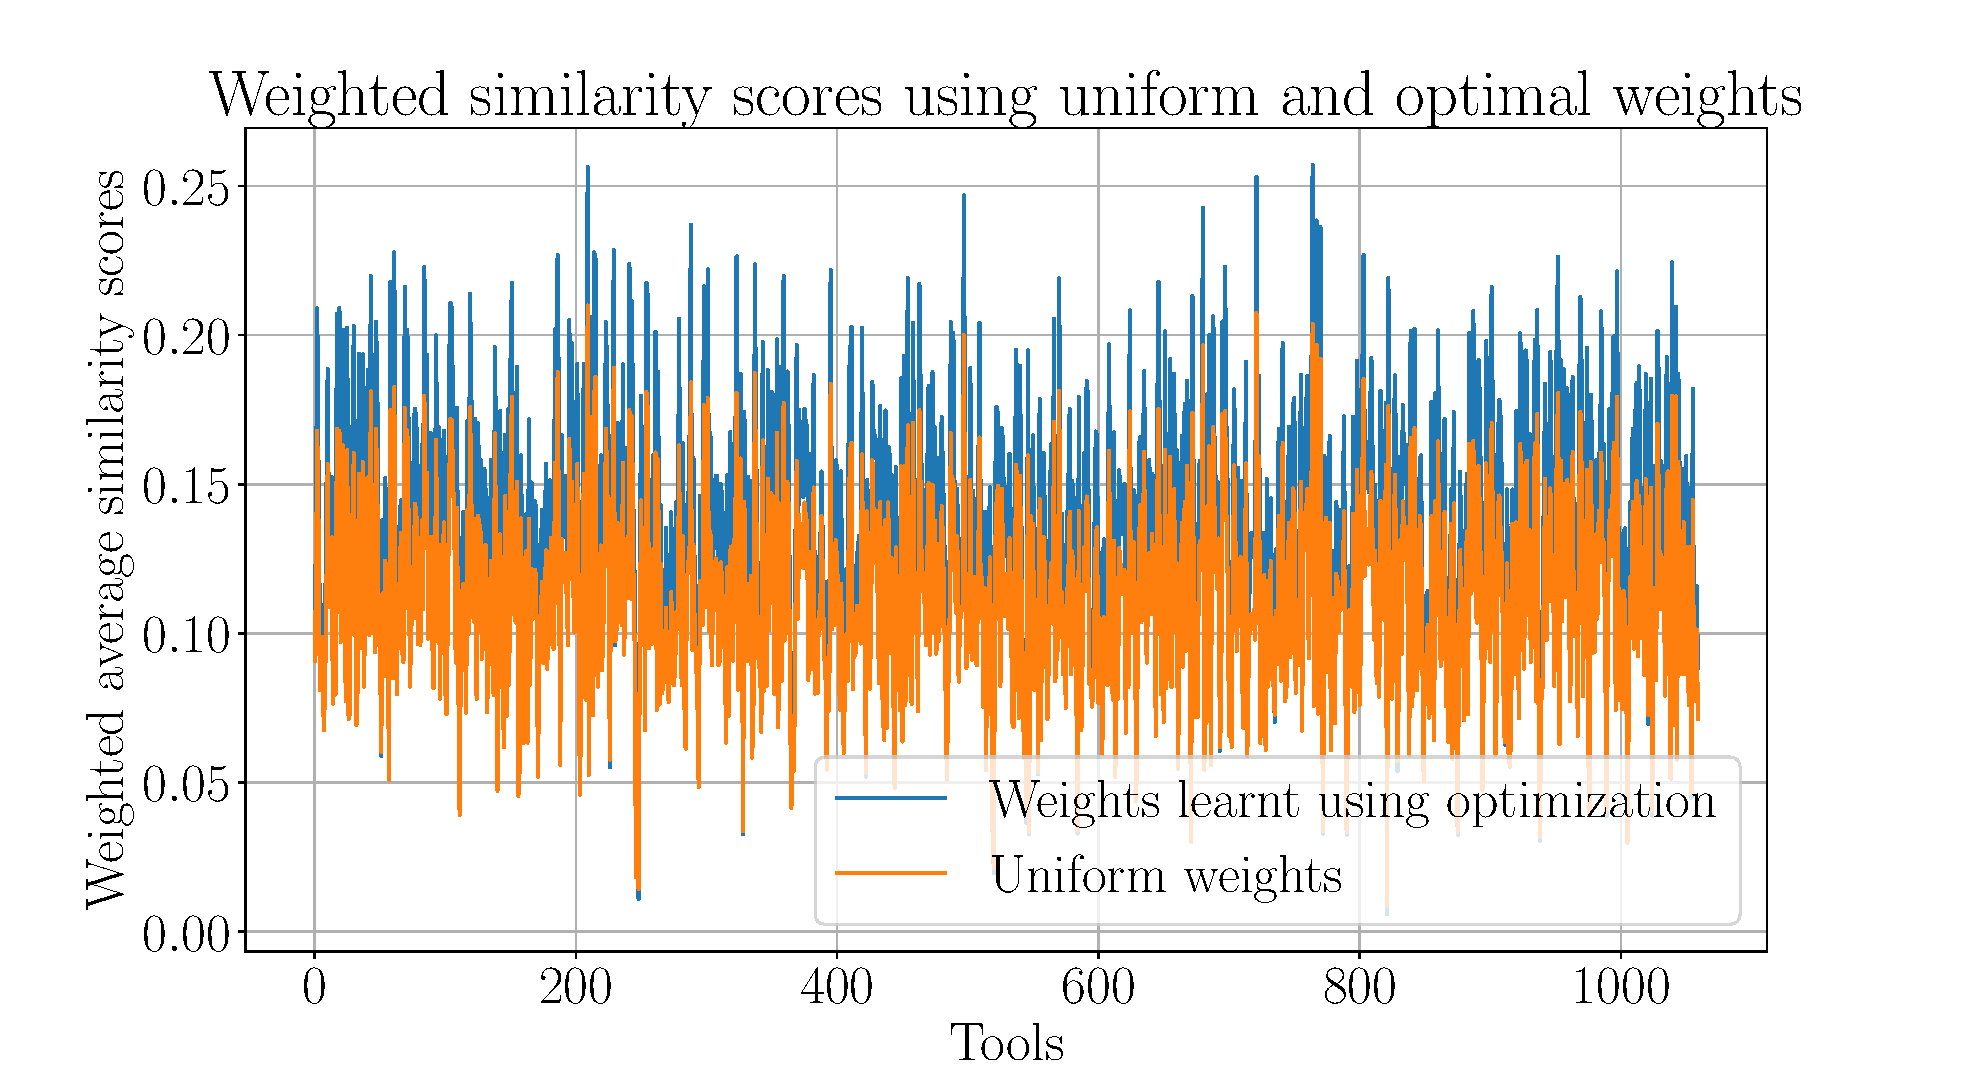
\includegraphics[scale=0.37]{figures/Optimization_005_lsi.pdf}}
    \caption[Average of uniformly and optimally weighted similarity scores computed using documents-tokens matrices reduced to $5\%$ of full-rank across all tools]{\textbf{Average of uniformly and optimally weighted similarity scores computed using documents-tokens matrices reduced to $5\%$ of full-rank across all tools}: The plot shows the average similarity scores where documents-tokens matrices reduced to $5\%$ of full-rank are used to compute similarity matrices and they are combined using uniform and optimal weights. We see that the average similarity scores computed using optimal weights are higher as compared to using uniform weights to compute similarity scores. Compared to figure 26, both the approaches, using uniform and optimal weights, measure higher similarity scores. }
\end{centering}
\end{figure}

\subsubsection{Static visualizer}
We created static html pages (visualizers) to look at the results. For latent semantic analysis approach, we have two such websites. In addition to showing similar tools for the selected tool, they show a few plots for the error, gradient and learning rate drop and the selected tool's similarity scores with all the other tools.

\begin{itemize}
\item Use full-rank documents-tokens matrices\footnote{\url{https://rawgit.com/anuprulez/similar_galaxy_tools/lsi/viz/similarity_viz.html}}
\item Use $5\%$ of full-rank documents-tokens matrices\footnote{\url{https://rawgit.com/anuprulez/similar_galaxy_tools/lsi_005/viz/similarity_viz.html}}
\end{itemize}

\section{Paragraph vectors}
We used paragraph vectors approach to learn fixed-length, multi-dimensional vectors for documents from name and description and help text. The figure 28 shows the documents-tokens matrices for input and output file types (28a), name and description (100-dimensional) (28b) and help text (200-dimensional) (28c). The matrices in 28b and 28c are dense. Using these matrices, we computed corresponding similarity matrices for the attributes (figure 29). We see that the similarity matrices are symmetric and dense. Due to this, the weight distribution also changes (figure 30). We learned higher weights for name and description (30b) and help text (30c) compared to input and output file types (30a). Figure 31 shows that the average similarity scores across all the tools are also higher compared to that of rank reduction approaches (figures 26 and 27). We increase the average similarity to $\approx0.30$ using optimal weights. For uniform weights as well, we record an average similarity of $\approx0.25$ (figure 31).

\subsubsection{Static visualizer}
For the paragraph vectors approach, the visualizer\footnote{\url{https://rawgit.com/anuprulez/similar_galaxy_tools/doc2vec/viz/similarity_viz.html}} shows similar tools by learning vectors for each document. In addition to showing similar tools for the selected tool, they show a few plots for the error, gradient and learning rate drop and the selected tool's similarity scores with all the other tools. 

\begin{figure}[h]
\begin{centering}
    {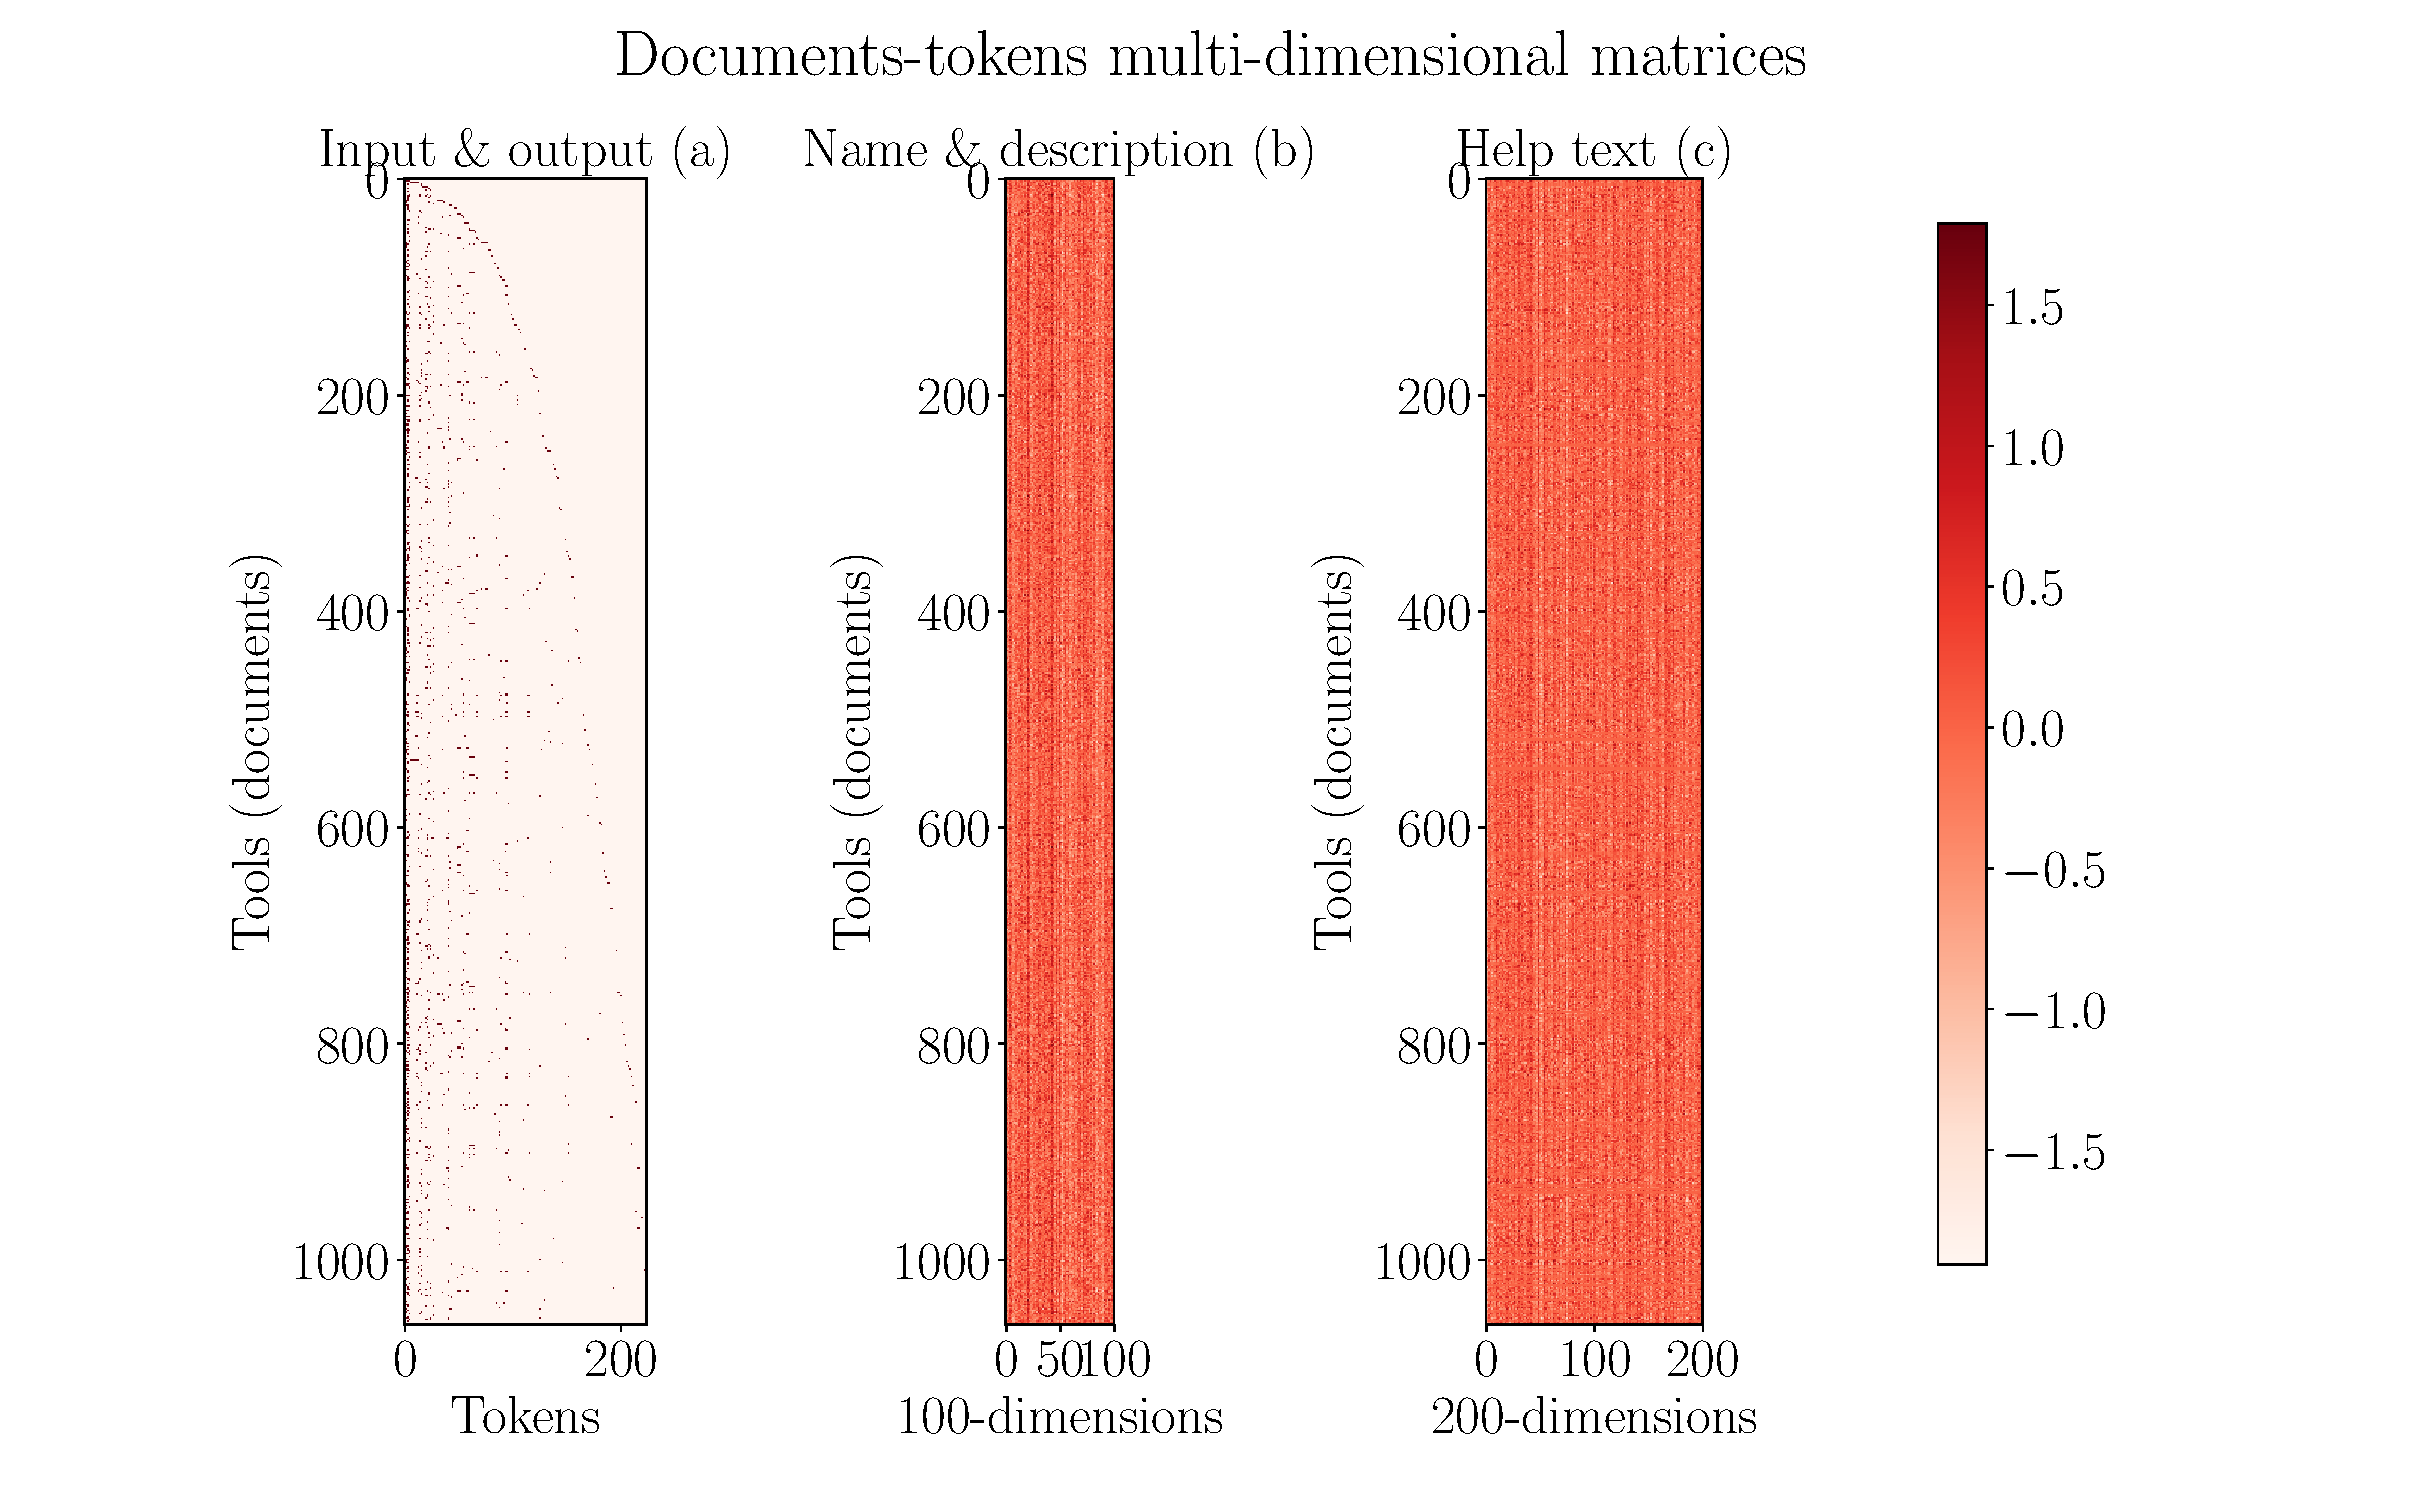
\includegraphics[scale=0.4]{figures/Documents-tokens_doc2vec.pdf}}
    \caption[Documents-tokens matrices for paragraph vectors approach]{\textbf{Documents-tokens matrices for paragraph vectors approach}: The heatmap shows documents-tokens matrices for input and output file types (a), name and description (b) and help text (c) attributes. The matrix in (a) is a document-token matrix where each entry shows a relative frequency of the token's occurrence. The matrices in (b) and (c) are 100 and 200 dimensional (each row is a document vector) respectively which means that each row of a matrix belongs to a document (paragraph) and is fixed-length and dense in nature. }
\end{centering}
\end{figure}

\begin{figure}[h]
\begin{centering}    
    {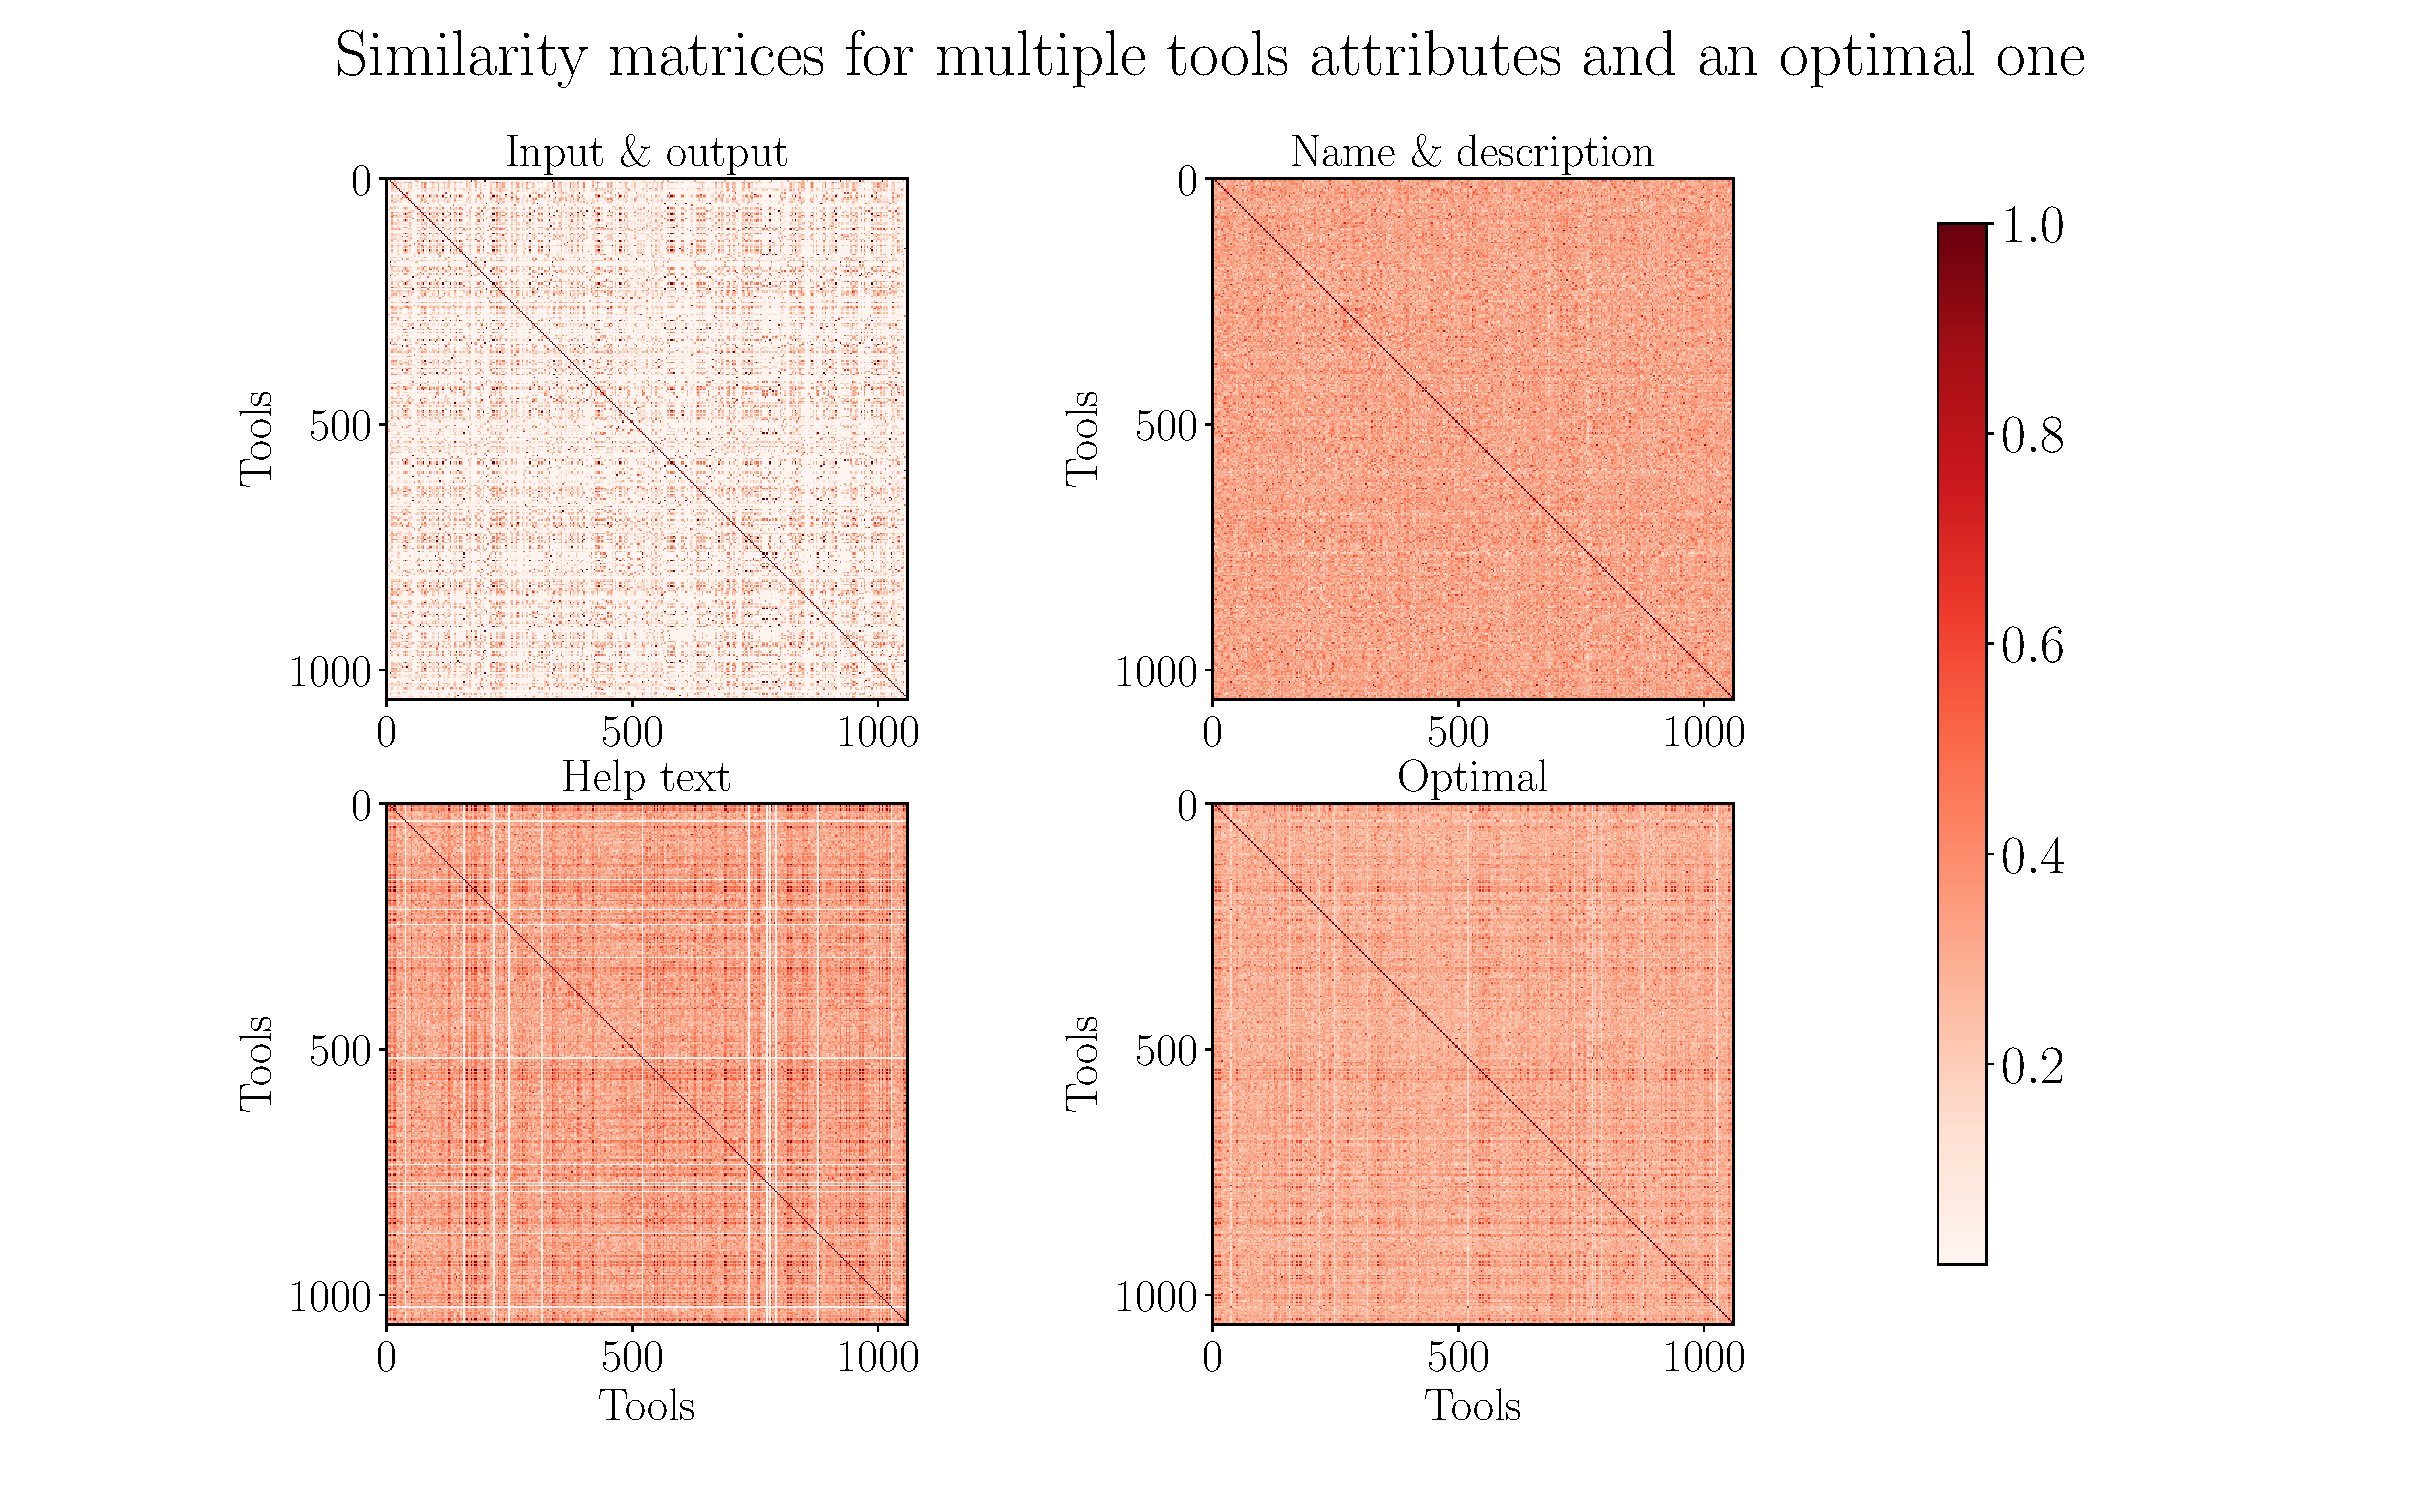
\includegraphics[scale=0.4]{figures/Similarity_matrices_doc2vec.pdf}}
    \caption[Similarity matrices using paragraph vectors approach]{\textbf{Similarity matrices using paragraph vectors approach}: The heatmap shows documents-documents (tools-tools) correlation matrices for input and output (a), name and description (b) and help text (c) attributes. The (d) shows a documents-documents (tools-tools) correlation matrix which is the weighted average computed using (a), (b) and (c) and weights (figure 22) given by the gradient descent optimizer (equation 15). The corresponding documents-tokens matrices are computed as shown in figure 28. The similarity matrices (b), (c) and (d) are denser compared to those from figure 23.}
\end{centering}
\end{figure}

\begin{figure}[h]
\begin{centering}
    {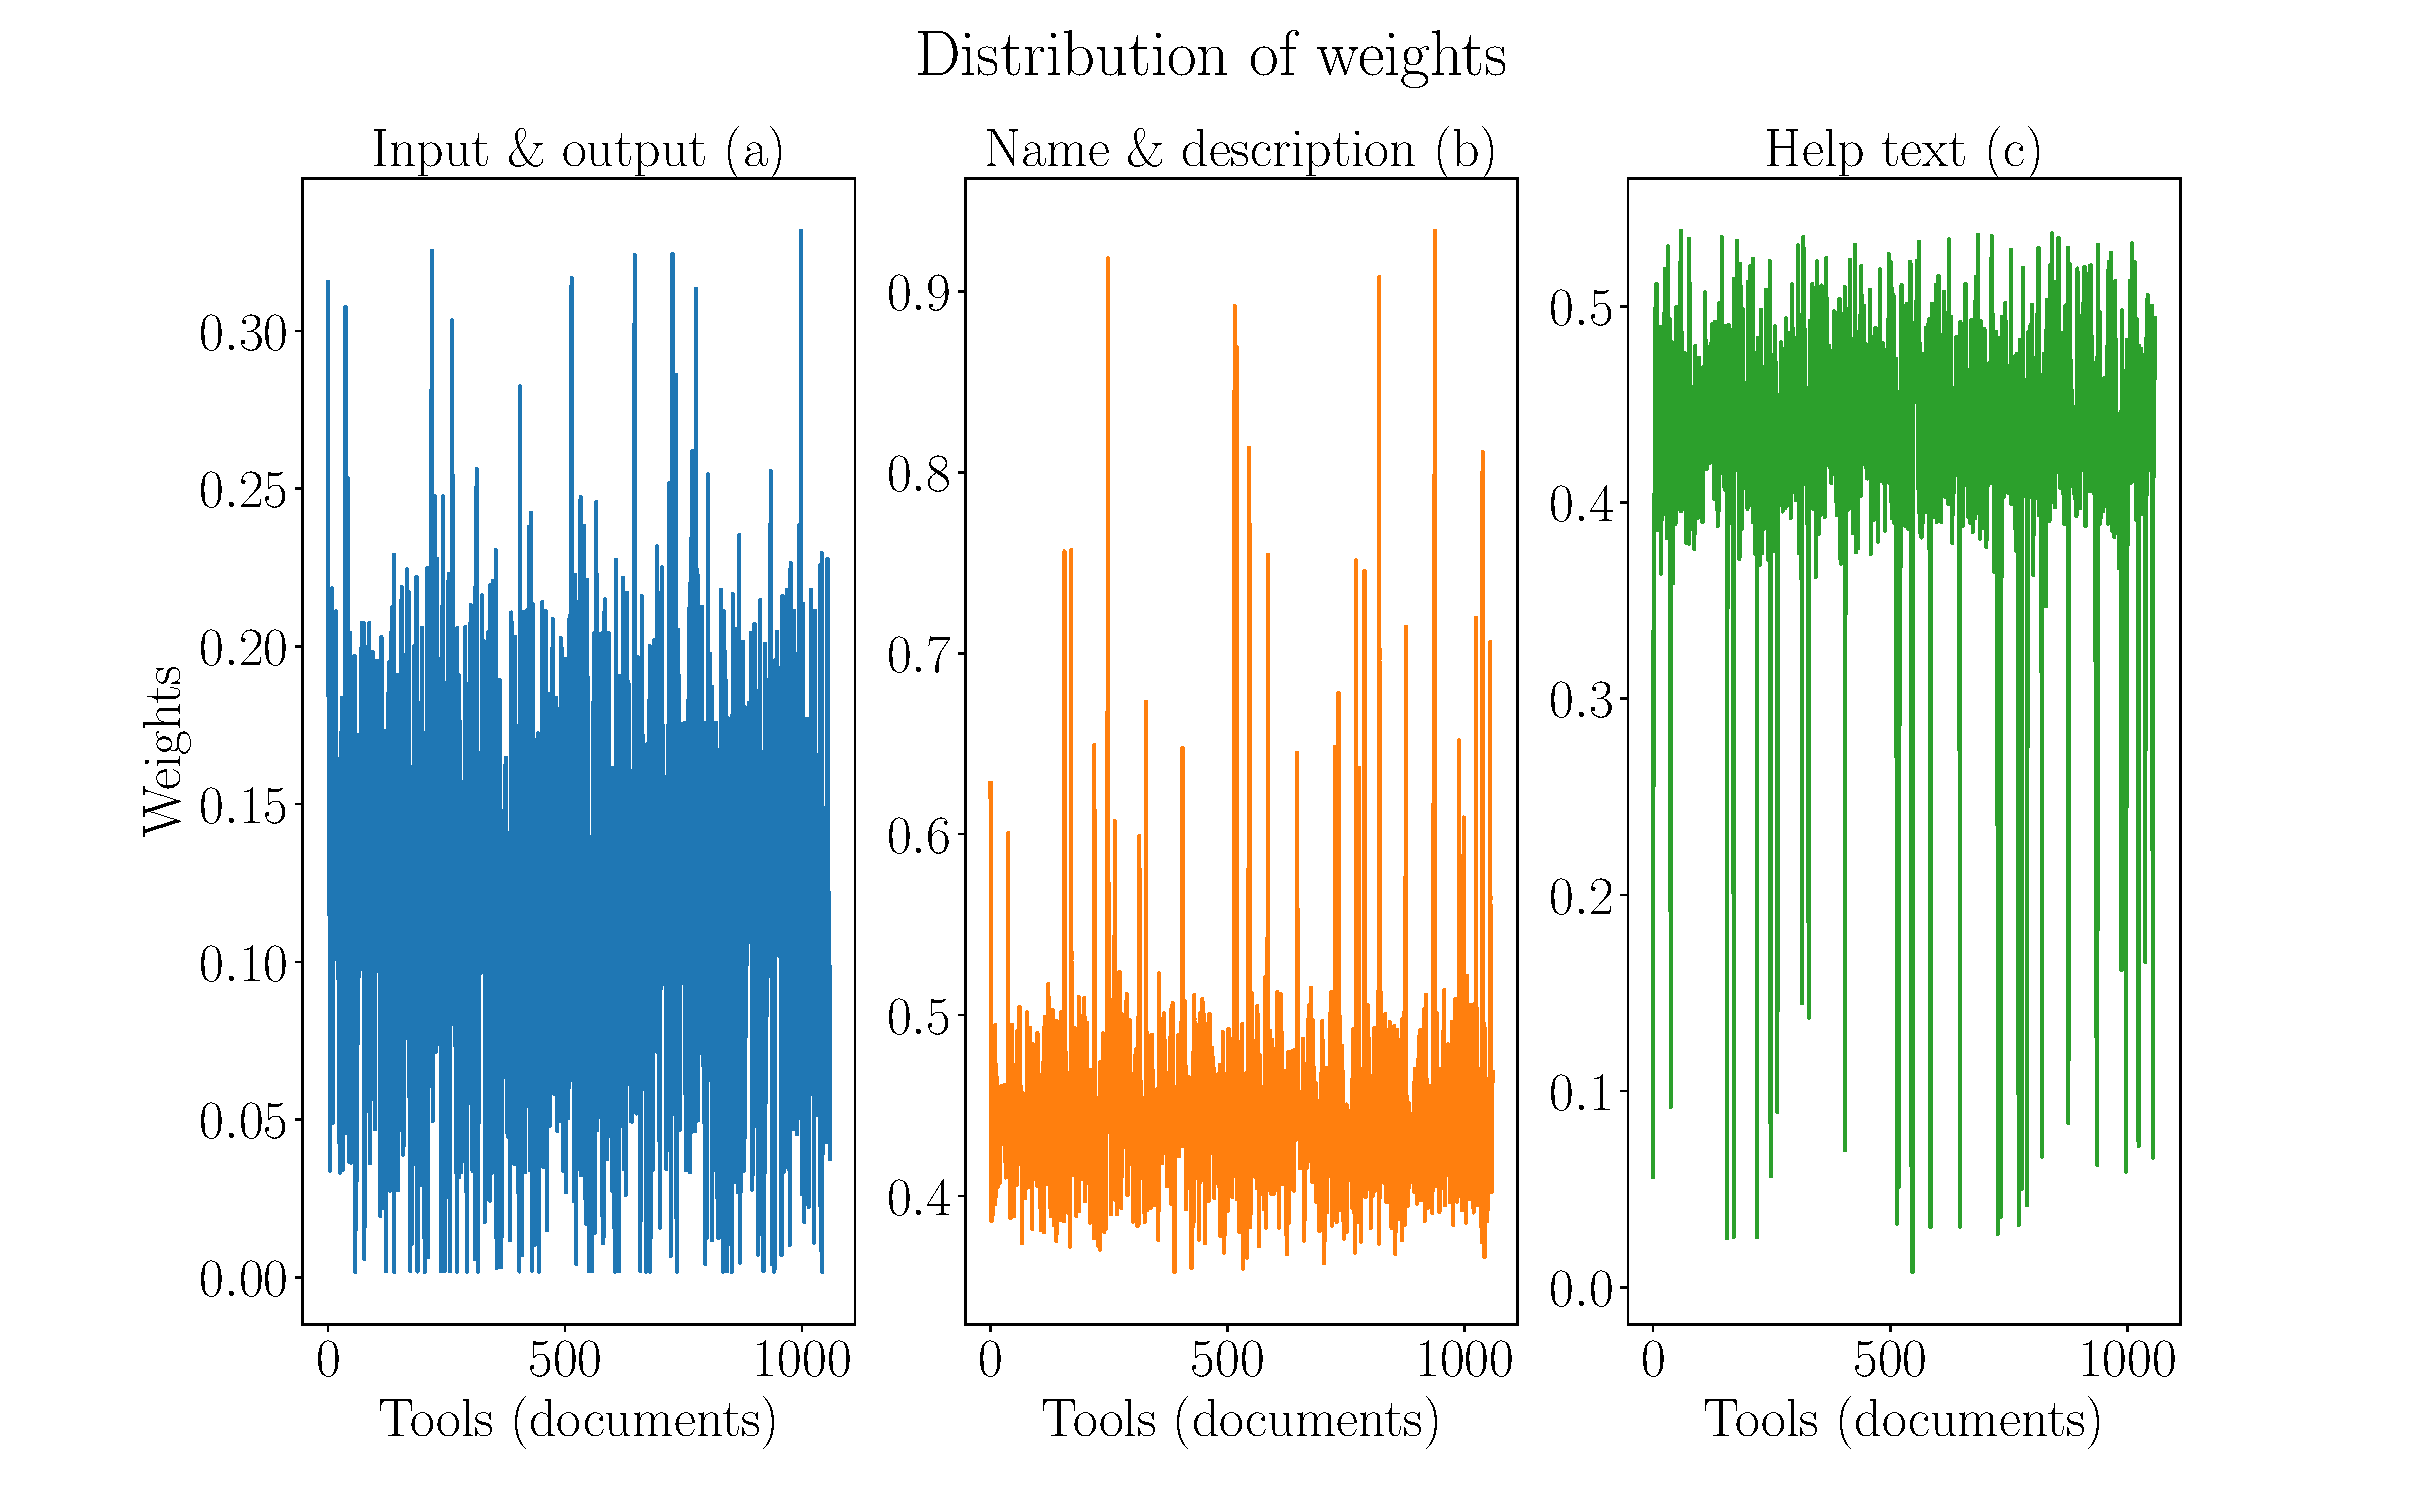
\includegraphics[scale=0.37]{figures/Weights_doc2vec.pdf}}
    \caption[Distribution of weights for similarity matrices computed using documents-tokens matrices for paragraph vectors approach]{\textbf{Distribution of weights for similarity matrices computed using documents-tokens matrices for paragraph vectors approach}: The plot shows the distribution of weights learned by gradient descent optimizer on the similarity matrices (29a, 29b and 29c) for the input and output file types (a), name and description (b) and help text (c) attributes. The corresponding documents-tokens matrices are computed as shown in figure 28.}
\end{centering}
\end{figure}

\begin{figure}[h]
\begin{centering}
    {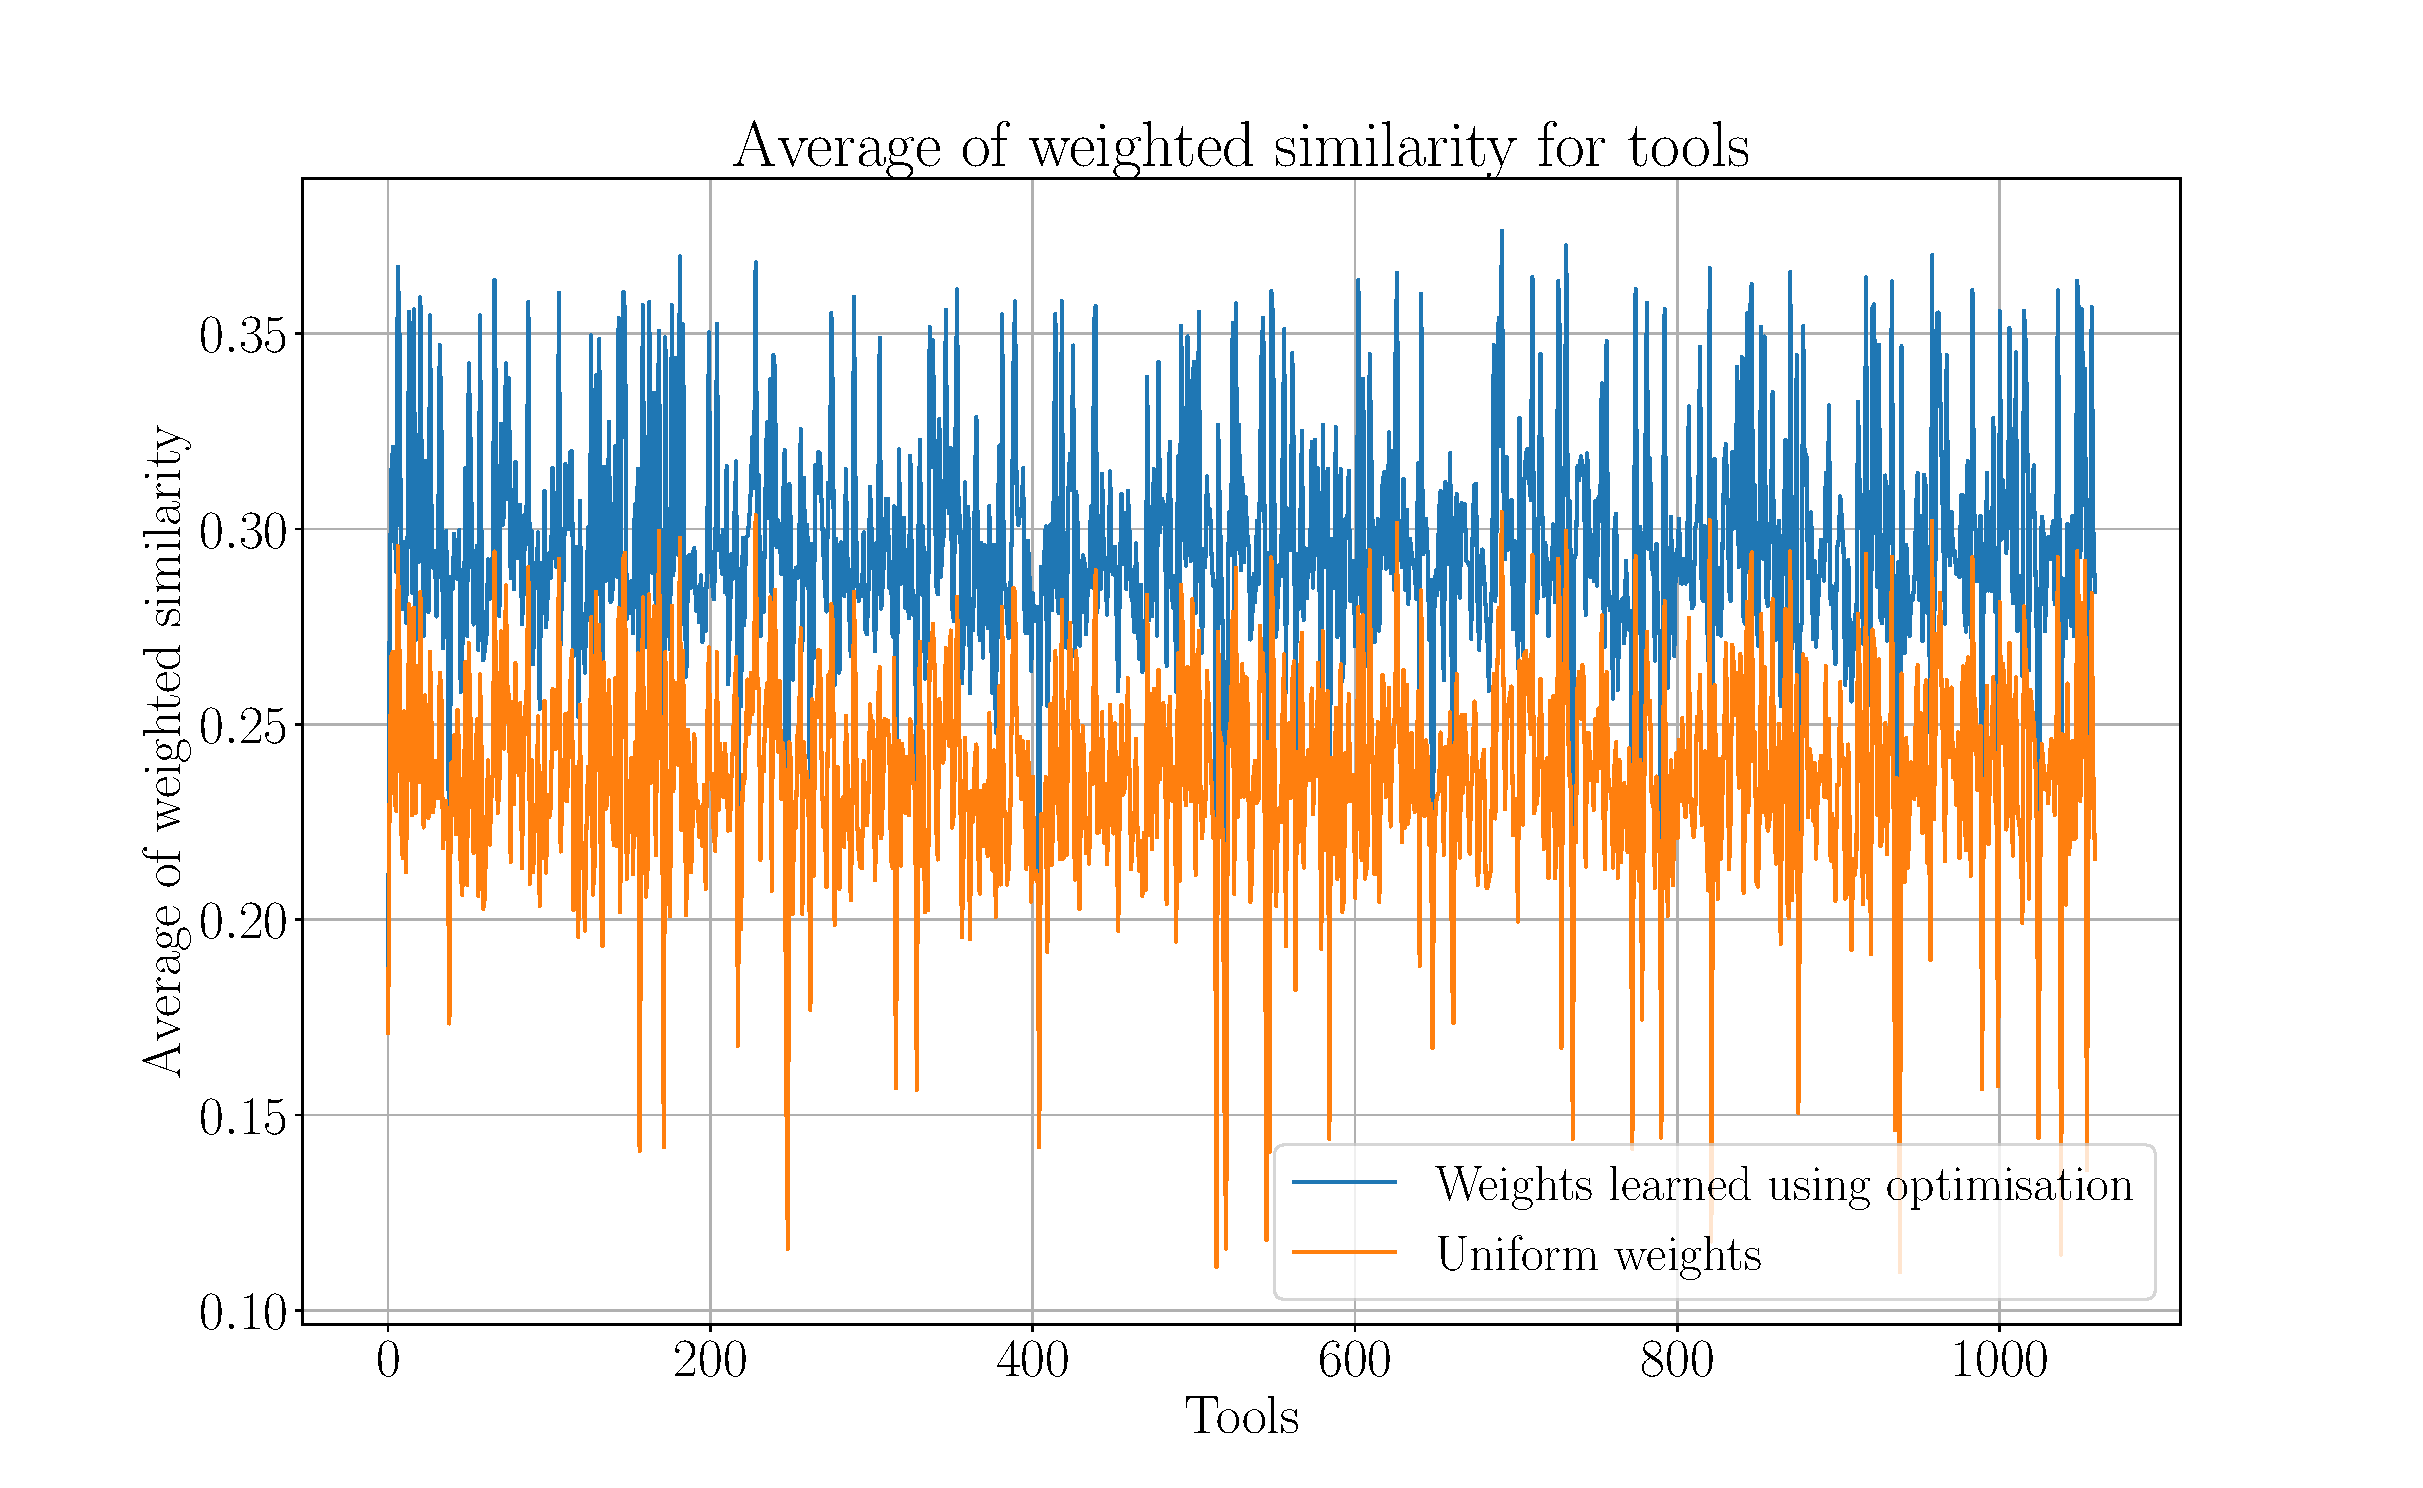
\includegraphics[scale=0.37]{figures/weighted_optimal_uniform_scores_pv.pdf}}
    \caption[Average of uniformly and optimally weighted similarity scores across all tools for paragraph vectors approach]{\textbf{Average of uniformly and optimally weighted similarity scores across all tools for paragraph vectors approach}: The plot shows a comparison of average similarity scores computed using weights learned using optimization and uniform weights across all tools. We can see that the average similarity scores using optimal weights are higher than using uniform weights. We can conclude that the optimizer learns higher weights on those similarity scores which are higher in magnitude. It learns higher similarity scores compared to latent semantic analysis approach (figure 26 and 27).}
\end{centering}
\end{figure}

\begin{figure}[h]
\begin{centering}
    {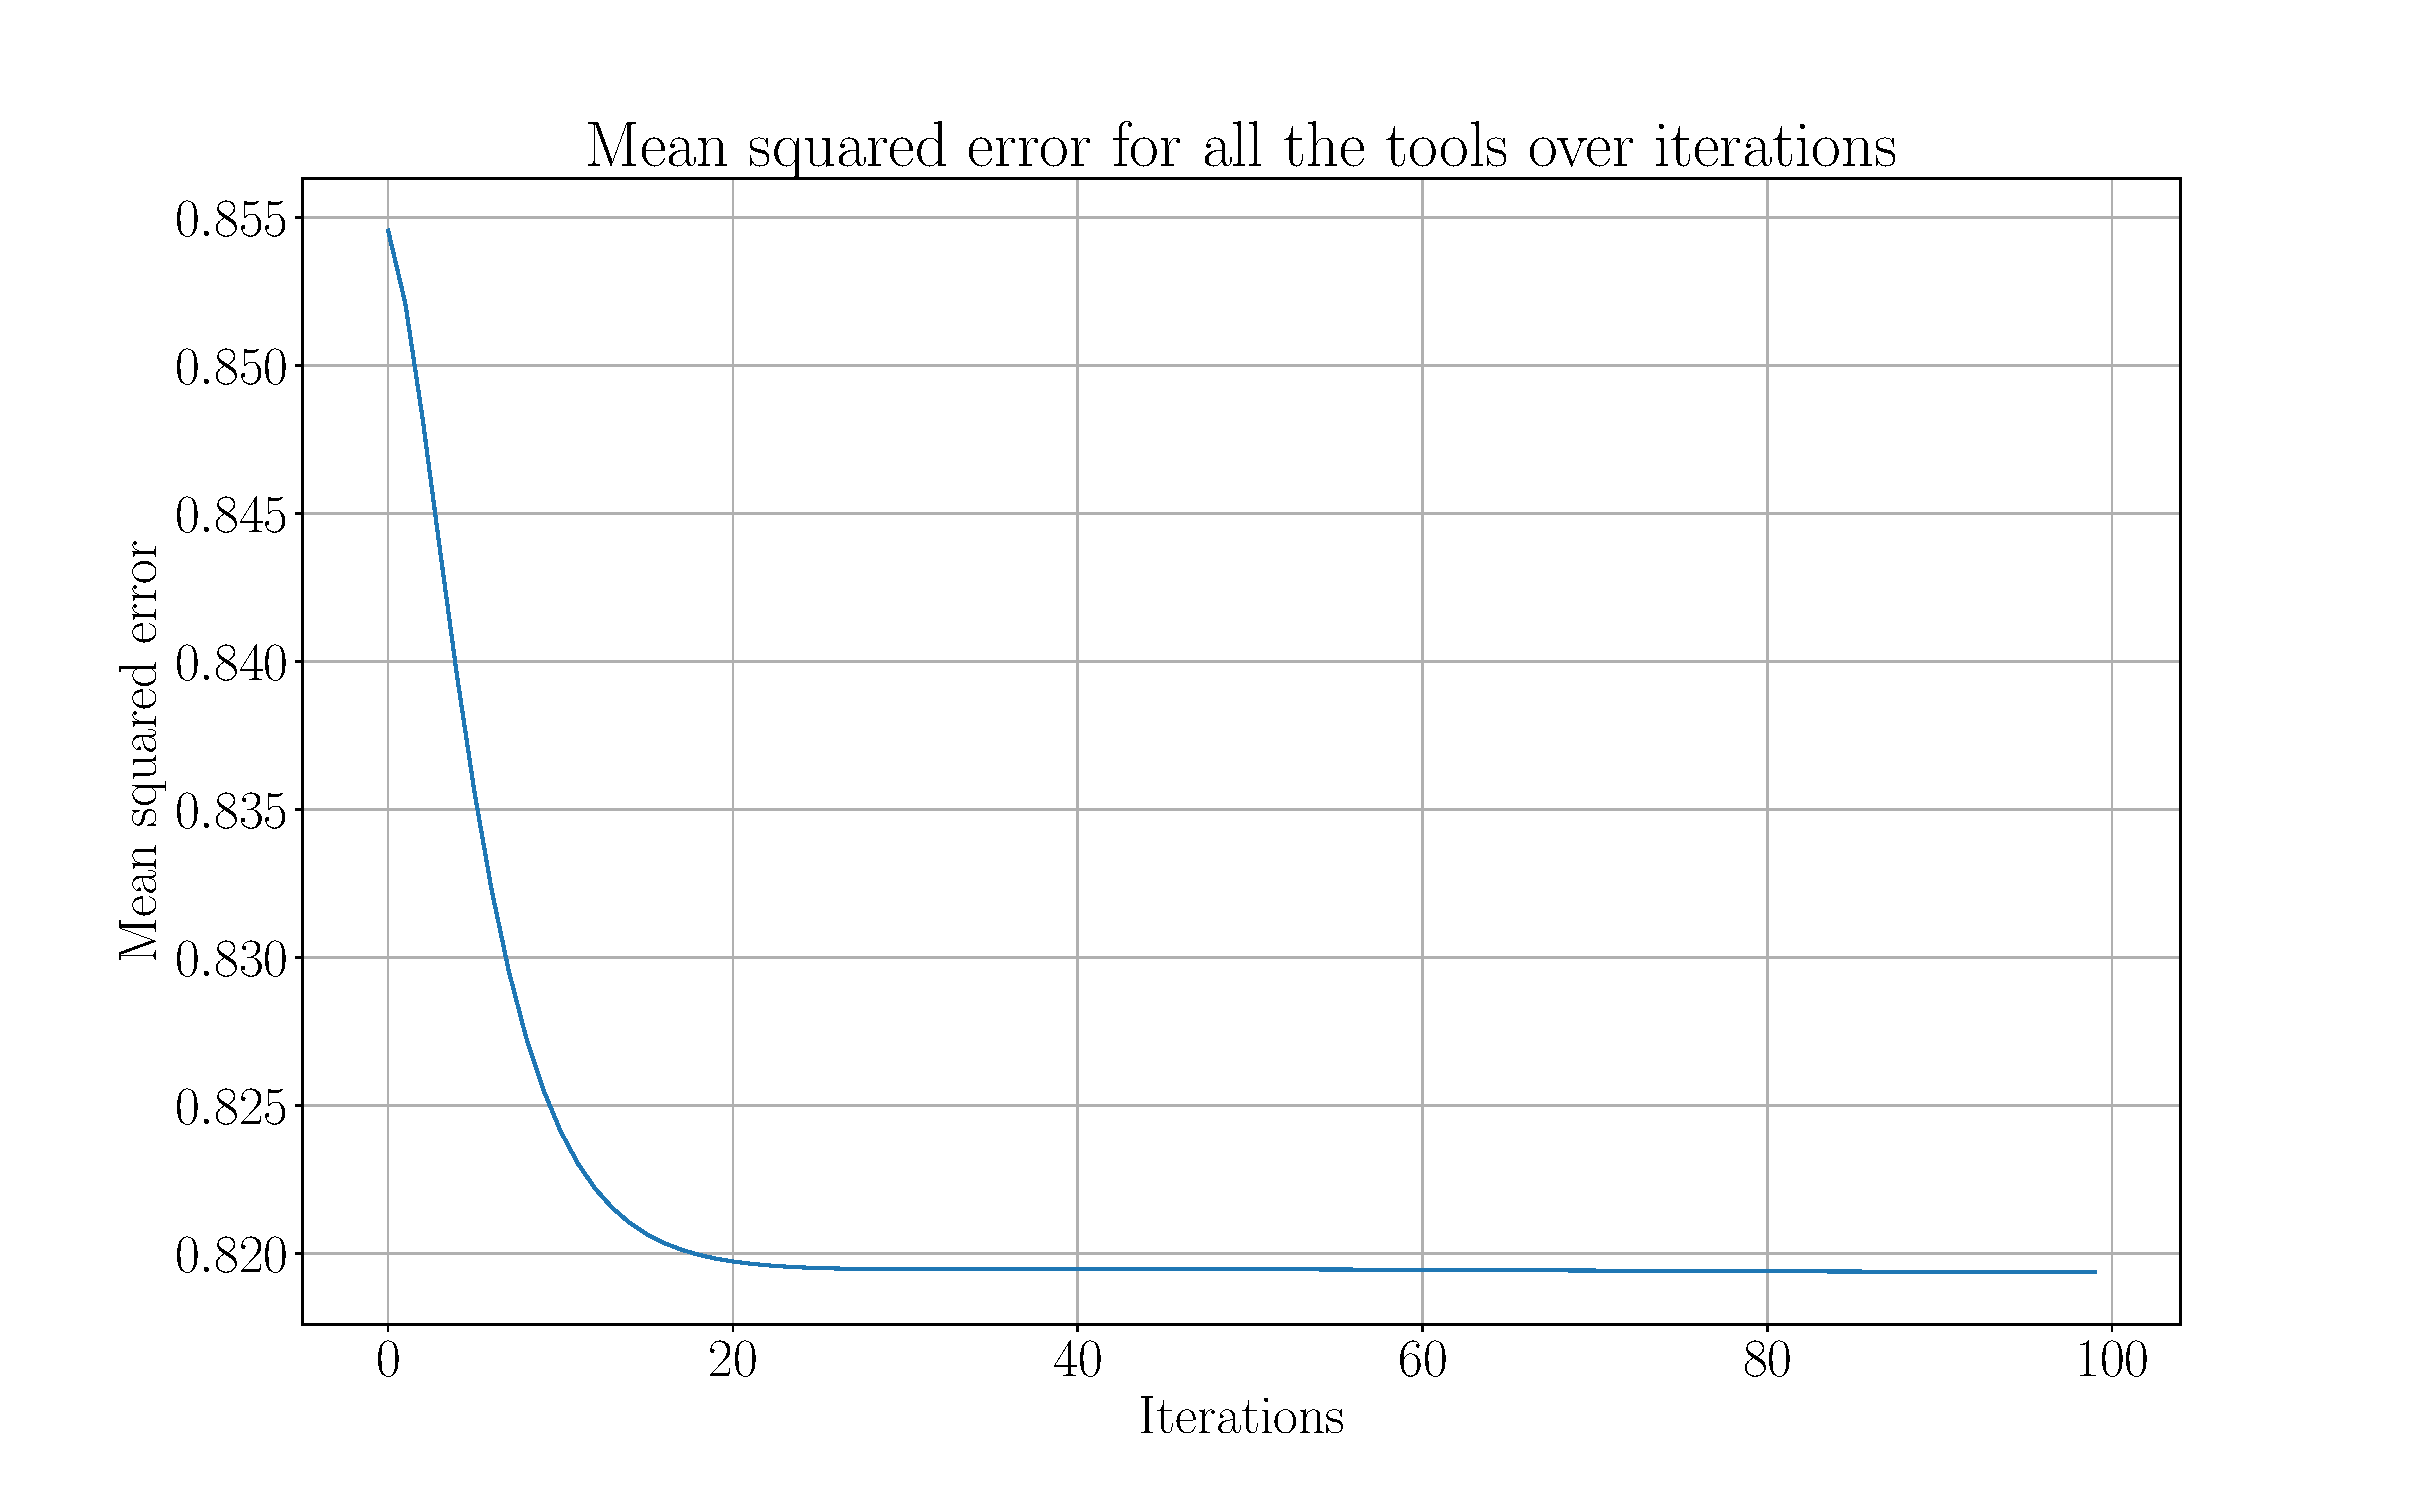
\includegraphics[scale=0.37]{figures/MSE_iterations_PV.pdf}}
    \caption[Mean squared error across all tools over iterations for paragraph vectors approach]{\textbf{Mean squared error across all tools over iterations for paragraph vectors approach}: The plot shows a drop in the mean squared error across all the tools and attributes over gradient descent iterations. As we move along the iterations, the error drops and stabilizes at $\approx30^{th}$ iteration.}
\end{centering}
\end{figure}

\section{Comparison of latent semantic analysis and paragraph vectors approaches}
We see a small case study in this section comparing the two approaches - latent semantic analysis and paragraph vectors using actual similarity values and weights learned for a tool "hisat". We find the similar tools for "hisat", a popular mapping tool, at the different stages of rank reduction and verify if we actually fetch the similar tools. We find similar tools once with full-rank documents-tokens matrices (table 2) and then with $5\%$ of full-rank documents-tokens matrices (table 3). In the end, we find similar tools for "hisat" using paragraph vectors approach (table 4) as well and compare them with the previous approaches. In the tables 2, 3 and 4, we look at the top-2 similar tools for "hisat" with their respective similarity scores for different attributes. The text below each table also gives the values of optimal weights. For example, the weighted similarity score in the first row of table 2 is calculated using the following equation (equation 30). The weights are given at the end of the table's description.

\begin{equation}
0.38 \cdot 0.77 + 0.10 \cdot 0.07 + 0.13 \cdot 1.0 = 0.42
\end{equation}

From the tables 2,3 and 4, we can say that the paragraph vectors approach works better than the latent semantic approach to find relevant similar tools by assigning reasonable similarity scores and learning optimal weights on them. In table 3, the similarity scores for name and description are not correct in the true sense as they measure $1.0$ even though their descriptions are not exactly same (overfitting). For table 2 in name and description column, they are way too less ($0.07$ and $0.12$). These incorrect interpretations would lead to wrong similarity assessment. Since we do not compute low-rank estimation of input and output file types matrix, its score remains same in table 2 and 3. In table 4, "hisat2" has the same score in all the tables (2,3 and 4). In table 4, the tool ranked at number two is more relevant than that from tables 2 and 3.

\begin{table}[ht]
\begin{center}
    \begin{tabular}{|l|l|l|l|l|}
        \hline
        Similar tools & input \& output & name \& desc. & help text & weighted similarity \\ \hline
        hisat2   & 0.38 & 0.07 & 1 & 0.42  \\ \hline
        srma\_wrapper & 0.5 & 0.12 & 0.01 & 0.4 \\ \hline
    \end{tabular}
    \end{center}
    \caption[Similar tools (top-2) for "hisat" extracted using full-rank documents-tokens matrices]{\textbf{Similar tools (top-2) for "hisat" extracted using full-rank documents-tokens matrices}: The table shows top-2 similar tools selected for "hisat". This set of similar tools uses full-rank documents-tokens matrices. The weights learned by optimization are 0.77 (input and output file types), 0.10 (name and description) and 0.13 (help text). }
    \label{tab:accuracy}
\end{table}

\begin{table}[ht]
\begin{center}
    \begin{tabular}{|l|l|l|l|l|}
        \hline
        Similar tools   & input \& output & name \& desc. & help text & weighted similarity \\ \hline
        hisat2   & 0.38 & 1 & 1 & 0.83 \\ \hline
        srma\_wrapper & 0.5 & 1 & 0.64 & 0.69 \\ \hline
    \end{tabular}
    \end{center}
    \caption[Similar tools (top-2) for "hisat" extracted using documents-tokens matrices reduced to 5\% of full-rank]{\textbf{Similar tools (top-2) for "hisat" extracted using documents-tokens matrices reduced to 5\% of full-rank}: The table shows top-2 similar tools selected for "hisat". This set of similar tools uses documents-tokens matrices reduced to 5\% of full-rank. The weights learned by optimization are 0.27 (input and output file types), 0.23 (name and description) and 0.5 (help text).}
    \label{tab:accuracy}
\end{table}

\begin{table}[ht]
\begin{center}
    \begin{tabular}{|l|l|l|l|l|}
        \hline
        Similar tools   & input \& output & name \& desc. & help text & weighted similarity \\ \hline
        hisat2   & 0.38 & 0.46 & 1 & 0.67 \\ \hline
        tophat & 0.25 & 0.73 & 0.54 & 0.58 \\ \hline
    \end{tabular}
    \end{center}
    \caption[Similar tools (top-2) for "hisat" extracted using paragraph vectors approach]{\textbf{Similar tools (top-2) for "hisat" extracted using paragraph vectors approach}: The table shows top-2 similar tools selected for "hisat". The weights learned by optimization are 0.14 (input and output file types), 0.44 (name and description) and 0.42 (help text).}
    \label{tab:accuracy}
\end{table}